%\chapter{3HDM}
%

\renewcommand{\cleardoublepage}{}
\renewcommand{\clearpage}{}

\chapter{3HDM Model}
\label{ch:3HDM}

We can now move on to the analysis of a three Higgs Doublet Model (3HDM), specifically a minimal BGL-like (Branco-Grimus-Lavoura) 3HDM. 
% 
At the core this BGL treatment is a stabilizing $\mathrm{U}(1) \times \mathrm{Z}_2$ global flavor symmetry, such as presented in Refs.~\cite{Ludvig_Thesis,Ian_Thesis}.
%
Whose purpose is to keep in check flavor violating decays. 
%
Note that without this symmetry these processes would occur at tree-level. 
%
Once the model is properly introduced we continue towards our numerical discussions in a similar fashion as before. 
%
Note, the simulations created for this model used a newer version of the previously discussed code containing the addition of a flavor calculation process based on python3 package entitled \texttt{flavio} \cite{straub2018flavio} and the inclusion of the Higgs alignment limit as to improve the scanning apparatus capabilities and ensure proper gauge couplings to a SM-like Higgs boson.
%
%{ \color{gray} This Higgs alignment process consists in forcing a CP-even eigenstate to serve as the observed Higgs Boson and give it precisely 125.09 GeV mass. This inversion process is achieved trough the translation of all Lagrangian terms relating to the Higgs sector in the gauge basis into physical parameters. } 
%
Note, a key change from the B-L-SM case is that the respective masses will all be calculated at tree-level instead of at 2-loop level. 
%
This is done for multiple reasons most of which reflect computational shortcomings and time constraints.
%
Note that radiative processes are still calculated correctly just using tree-level masses, e.g. the value of $(g-2)_\mu$ is still calculated by SPheno but for a tree-level set of masses.

%{ \color{gray} Our results show that light scalars are still within the reach of future collider experiments in our models framework while having FCNCs concurrent with observations.  
%
%Given these conclusions we also performed a additional as to check if accidental fine-tuning was present in our results, possibly due to a random synchronicity discovered in the Monte-Carlo scan.
%
%To do this we varied all the soft breaking terms for the collected data by 1\% of their original value disregarding the effects this will have for the alignment of the Higgs. 
%
%In the validated parameter space by all other constraints we found no significant sensitivity to mass variation.  
%
%Furthermore for completeness we also implemented a \texttt{MadGraph5\_aMC@NLO 2.6.2} routine as to probe future detection of these light scalars in newer collider experiments and discovered there is still regions that are far from discovery.  \color{blue} maybe conclusions? }  

\section{The Case of the BGL-2HDM and its Relation to our Work}


Any 3HDM can be thought of as part of a larger family of multiple Higgs Doublet Models, or NHDMs, the first iteration of which was the Two Higgs Doublet Model (2HDM) proposed by T.D. Lee \cite{Lee1973}. At the time, Lee was motivated by the search for a spontaneous breaking of the CP symmetry which was included in his model.  However the 2HDM quickly became a very popular model motivated by it's inclusion for dark matter candidates, as well as providing a large particle spectrum, including charged and additional neutral scalars who enable FCNC deviations. In spite of the fact that, now, these tree-level FCNCs are in direct opposition to experimental results, as discussed in section \ref{Chap_1_Sec_3}. Given these limits, we can consult the literature, as in Ref. \cite{Branco:1999fs}, and see that the existence of FCNCs forces the extra scalars in the minimal 2HDM case to have masses above 1 TeV as to suppress FCNCs. These heavy scalars are far from ideal, since there is no indication such heavy scalars exist nor do they provide us with interesting physics. 

Several mechanisms have been proposed to deal with suppression of these tree-level FCNCs as to allow for richer physics and lighter scalars. First, in Ref. \cite{ferreira2019strong}, it is proposed a framework in which we have the balancing of CP-odd and CP-even contribution to FCNCs, however, this requires some fine-tuning, making it very unappealing based on a ``naturalist" argument. Another possibility is to assume alignment between different Yukawa matrices such that no FCNCs are present, see \cite{Jung_2011}. Finally we could also use the approach presented in the BGL version of the 2HDM \cite{Branco_1996}, here the authors impose a flavor-violating symmetry naturally keeping the FCNCs under control trough the CKM matrix. The phenomenology of the model has been studied quite thoroughly in previous works, see Ref. \cite{Botella_2016}, and it remains a possible scenario for BSM physics.

As the name indicates, NHDMs, are types of models where, in parallel with the standard SM Higgs doublet some additional replicas of that same  (or slightly modified) doublet are introduced. In the NHDM these form a sort of family in the scalar sector in analogy to the fermion sector. Being that the 3HDM is the most similar. This idea is far from original and was first discussed by Weinberg in Ref. \cite{Weinberg1976}.

Phenomenologically speaking these 2HDMs and 3HDMs models are quite different however, and we can argue that there are several advantages to the 3HDM. Such as, unlike in the 2HDM case, the 3HDM can provide more than one stable source of spontaneous CP symmetry breaking \cite{Branco_2012}. Furthermore, charge breaking minima were found to be stable while at the same time coexisting with charge-preserving ones (for more information see, \cite{Barroso_2006}). Note also, for the 2HDM a full list of all possible incorporation of symmetries consistent with $\mathrm{SU(2)}\times\mathrm{U(1)}$ has been achieved \cite{Ivanov_2008}, while for the 3HDM no work has thus far been completed, see, \cite{Ivanov_2015}. 

In this work we explore a 3HDM with a global flavor symmetry to replicate the BGL treatment. And in fact similar studies have been done in 3HDMs that include different flavor symmetries, such as Ref.\,\cite{Camargo_Molina_2018}. Given this background it is no surprise that we will focus particularly in the measuring Quark Flavor Violation (QFV) observables. In our analysis these will consist of meson decays or oscillations that include the changing of quark flavor within the meson. These QFV observables will be compared to measured amplitudes in collider experiments as to offer a novel exclusion to our model. Note, the additional flavor symmetry constrains the terms that can appear in the Yukawa sector of the Lagrangian resulting in very specific structures (or textures) of the Yukawa couplings. These shapes generate a suppression mechanism trough the CKM matrix off-diagonal terms restricting the values of FCNCs in our model.%


 
\section{The formulation of a BGL-like 3HDM} 

Again, for this model, we still retain most of the same fields with equal charges as we saw under the $\mathcal{G}_{SM}$ in the SM chapter~\ref{Chap:SM}. These fields are seen in, 
%
\begin{equation}
\label{eq:3HDM_Fields}
\begin{gathered}
Q_{L_i} =  \begin{pmatrix}
u_{L_i}  \\
d_{L_i}
\end{pmatrix} \quad , \quad \Psi_{L_i} =  \begin{pmatrix}
\nu_{L_i}  \\
e_{L_i}
\end{pmatrix}  ,  \\ 
p_R \quad , \quad n_R \quad , \quad e_{R_i} \quad i=\{1,2,3\}  ,  \\  
\phi_k = \begin{pmatrix}
W_k^\pm + i \, W_k^\mp \\ 
\frac{1}{\sqrt{2}}\left( v_k + h_k + i Z_k \right) 
\end{pmatrix}  \quad , \quad k=\{ 1,2,3\}  . 
\end{gathered} 
\end{equation}
%
where $Q_{L_i}$ , $\phi_k$ and $\Psi_{L_i}$ are $\mathrm{SU(2)_L}$ doublets while, $p$ and $n$ (these are analogous to $u_{R_i}$, $d_{R_i}$ in the SM respectively), and $e_{R_i}$ are $\mathrm{SU(2)_L}$ singlets where the i and k generation stand for their respective generation indexes. 
%
Where the new charges under $\mathrm{U(1)}\times\mathbb{Z}_2$ can be seen in the transformations that these fields undergo, 
%
\begin{equation}
\label{eq:3HDM_Transformations}
	\begin{split} 
	\mathrm{U(1)} : & \\
		& Q_{L_3} \rightarrow    e^{i \alpha} Q_{L_3}  \\  
		& p_{R_3} \rightarrow    e^{2 i \alpha} p_{R_3}  \\
		& \phi_1  \rightarrow    e^{i \alpha} \phi_1  \\   
		& \Psi_{L_1} \rightarrow e^{i \alpha} \Psi_{L_1} \\
		& \phi_3 \rightarrow     e^{i \alpha} \phi_3  \\ 
	\end{split} \quad \quad \quad  
	\begin{split}
		\mathbb{Z}_2 : & \\
		 	& Q_{L_3} \rightarrow -Q_{L_3} \\
		 	& p_{R_3} \rightarrow -p_{R_3} \\ 
		 	& \phi_1  \rightarrow -\phi_1 \\ 
		 	& \Psi_{L_1} \rightarrow - \Psi_{L_1} \\ 
		 	& \phi_3 \rightarrow -\phi_3
	\end{split}  
\end{equation} 
%
All remaining fields not shown in Eq. \ref{eq:3HDM_Transformations} remain unchanged under transformations of the $\mathrm{U(1)}\times\mathbb{Z}_2$ global symmetry i.e. are not charged under these symmetries.  
%
Note there is no right handed neutrino fields in this model making it so that no neutrino mass terms appear unlike in the case of the B-L-SM.

\subsection{The Scalar Sector}

Let us then start our proper introduction to the workings of the model by presenting the scalar sector where the new spin-0 $\mathrm{SU(2)}$ doublets, $\phi_k$, $k=\{1,2,3\}$ reside.
%
Note the scalar potential is $\mathcal{CP}$-invariant, this means, 
%
\begin{equation}
\phi_1 = \phi_1^{\**} \quad , \quad \phi_2 = \phi_2^{\**} \quad , \quad 
\phi_3 = \phi_3^{\**} . 
\end{equation}
% { \color{red} Não falta um sinal de menos no $\phi_{1,3}$ Eu disse que o outro não se transforma sobre Z2 mas como isto é CP trans. não devia de ter? Ask morais } 
%
The generic scalar potential is extensively written in, 
\begin{equation}
\label{eq:3HDM_Scalar_Pot}
\begin{split}
V(\phi_i) = & 
- \mu_1^2 \left( \phi^{\dagger}_1 \phi_1 \right) 
- \mu_2^2 \left( \phi^{\dagger}_2 \phi_2 \right)  
- \mu_3^2 \left( \phi^{\dagger}_3 \phi_3 \right) \\ 
& \left[ - \mu_{21}^2 \left( \phi^{\dagger}_2 \phi_1  \right) 
  - \mu_{23}^2 \left( \phi^{\dagger}_2 \phi_3  \right)  
  - \mu_{13}^2 \left( \phi^{\dagger}_1 \phi_3  \right) + \text{H.c.} \right]  \\
& + \lambda_1 \left( \phi^{\dagger}_1 \phi_1 \right) 
  + \lambda_2 \left( \phi^{\dagger}_2 \phi_2 \right)  
  + \lambda_3 \left( \phi^{\dagger}_3 \phi_3 \right) \\  
& + \lambda_4 \left( \phi^{\dagger}_1 \phi_1 \right)  \left( \phi^{\dagger}_2 \phi_2 \right) 
  + \lambda_5 \left( \phi^{\dagger}_1 \phi_1 \right)  \left( \phi^{\dagger}_3 \phi_3 \right)  
  + \lambda_6 \left( \phi^{\dagger}_2 \phi_2 \right)  \left( \phi^{\dagger}_3 \phi_3 \right)  \\ 
& + \lambda_7 \left( \phi^{\dagger}_1 \phi_2 \right)  \left( \phi^{\dagger}_1 \phi_2 \right)  
  + \lambda_8 \left( \phi^{\dagger}_1 \phi_3 \right)  \left( \phi^{\dagger}_3 \phi_1 \right)   
  + \lambda_9 \left( \phi^{\dagger}_2 \phi_3 \right)  \left( \phi^{\dagger}_3 \phi_2 \right)  \\
& + \lambda_{10} \Bigg\{ \left( \phi^{\dagger}_1 \phi_3 \right)^2 + \text{H.c.} \Bigg\} . 
\end{split} 
\end{equation}
%
%{ \color{red} Este potencial tem de ser visto com cuidado. Primeiro, os termos com $\lambda_{1,2,3}$ são iguais aos termos com $\mu^2_{1,2,3}$ mas com o simal trocado. Segundo, porque que é que o $\lambda_{10}$ é o único com Hermıitico conjugado? Não estamos a fazer double counting com isto} 
%
Due to the $\mathcal{CP}$ symmetry imposed on this potential all parameters, $(\lambda_i,i=\{1,...,10\})$ and soft-breaking terms, here are real.
%
The most generic version of this soft breaking is given by the second line, where the soft-breaking terms $\mu_{23}^2$, $\mu_{13}^2$ and $\mu_{21}^2$ are seen. 
%
The parameter $\mu_{23}^2$, is necessarily added as to impede the formation of a massless axion and is the only term that respect the $\mathbb{Z}_2$ symmetry while the others explicitly break it. Note the  $\mathrm{U(1)}$ portion is broken explicitly by all these terms. 
%
%{\color{red} Porque? Todos os termos da segunda linha são genéricos de um potential 3HDM. Não? e porque nao introduzir mais só estes termos quebram a symmetry imposta?} 
%
%Of these note that the $\mu^2_{23}$ term is the only one that respect the $\mathbb{Z}_2$ symmetry while the others also break $\mathrm{U(1)}$ portion. 
%
%A study of these parts of the flavor symmetry, has been included in the first analysis of Ref.~\ref{Ian_Thesis}.

After the process of SBB, all Higgs doublets, $\phi_k$, take a VEV shape similar to that of the SM Higgs, written as, 
%
\begin{equation}
\phi_k = 
\begin{pmatrix}
W_k^\pm + i \, W_k^\mp \\ 
\frac{1}{\sqrt{2}}\left( v_k + h_k + i Z_k \right)
\end{pmatrix}  \rightarrow \langle \phi_k \rangle = \begin{pmatrix}
0 \\ 
\frac{v_k}{\sqrt{2}}
\end{pmatrix} \quad , \quad k=\{ 1,2,3\} .  
\label{eq:3HDM_Higgs_Field_VEV} 
\end{equation} 
%
Here we see the charged portion of the field, $W_k^\pm$, the CP-odd portion, $Z_k$, and finally the CP-even, $h_k$. 
%
%Note that after SBB there will still remain 3 massless states (Goldstone bosons) that will be later absorbed into the gauge bosons $W$ and $Z$. 
%
%This allows for them to be removed from the scalar spectrum.

Recall that, for the given scalar potential $V$ as seen in Eq.\,(\ref{eq:3HDM_Scalar_Pot}) to have a stable vacuum it needs to satisfy the tadpole equations i.e. a unchanging potential ensuring that there is a absolute minimum of energy. 
%
To solve these one must write the derivatives of the potential with respect to the fields and then observe their values once the process of SBB occurs, this process yields the following equations,
%
\begin{equation}
\label{eq:3HDM_tadpoles}
\begin{split}
\frac{\partial V}{\partial \phi_1} = & \frac{1}{2} v_1 \left(-2 \mu _1^2+\left(\lambda _4+\lambda _7\right) v_1^2+\left(\lambda _5+\lambda _8+2 \lambda _{10}\right) v_7^2\right)+\lambda _1 v_1^3-\mu _{13}^2 v_3-\mu _{21}^2 v_2 \\ 
\frac{\partial V}{\partial \phi_2} = & \frac{1}{2} v_2^2 \left(-2 \mu _2^2+\left(\lambda _6+\lambda _9\right) v_3^2+\left(\lambda _4+\lambda _7\right) v_1\right)+\lambda _2 v_2^3-\mu _{21}^2 v_1-\mu _{23}^2 v_3 \\
\frac{\partial V}{\partial \phi_3} = & \frac{1}{2} \left(2 \lambda _3 v_3^3+\left(\lambda _6+\lambda _9\right) v_2^2 v_3+\left(\lambda _5+\lambda _8+2 \lambda _{10}\right) v_1^2 v_3-2 \mu _3^2 v_3-2 \mu _{13}^2 v_1-2 \mu _{23}^2 v_2\right) \\
\end{split} 
\end{equation}

\subsubsection{The Higgs Basis}

It is convenient for the remainder of our study to now introduce the basis changing matrix to what we will call the Higgs Basis.
%
In our analysis of the 3HDM we did not perform the conventional direct diagonalisation of the scalar and Yukawa bi-linear terms expressed in the scalar potential (Eq.\,(\ref{eq:3HDM_Scalar_Pot})) expanded around the vacuum state.
%
Instead we use a intermediate basis in between the process of expressing the mass eigenstates as to significantly simplifies the analysis of the scalar, pseudoscalar, charged scalar and quark physical terms 
%
%Instead of the direct diagonalisation that is often performed of the gauge basis mass forms extracted from the bi-linear terms of the potential see in Eq.\,\ref{eq:3HDM_Scalar_Pot}, expanded around the vacuum state, the use of the intermediate Higgs basis significantly simplifies the analysis of the scalar, pseudoscalar and the charged scalar sectors. 
%
e.g this base change will allow us to express the charge and pseudoscalar states in such a way as to become apparent that a Goldstone emerges in each case. 
%
These Goldstones will account for the longitudinal polarization of W and Z bosons. 

The transformation from the gauge to the Higgs basis reads, 
\begin{equation}
\mathcal{O} = 
\begin{pmatrix}
\dfrac{v}{v_1} & \dfrac{v}{v_2}  & \dfrac{v}{v_3} \\[1.2em]
\dfrac{v_3}{v_{13}} & 0 & \dfrac{-v_1}{v_{13}} \\[1.2em]
\dfrac{v_2 v_1}{v v_{13}}  & \dfrac{v_{13}}{v} & \dfrac{v_2 v_3}{v v_{13}}  
\end{pmatrix} , 
\end{equation}
%
where $v_{13}=\sqrt{v_1^2 + v_3^2}$ and $v=\sqrt{v_1^2 + v_2^2 + v_3^2 }$, the total magnitude. This basis transformation explicitly relate the fields in the following manner, 
%
\begin{equation}
\begin{pmatrix}
\phi_1 \\
\phi_2 \\
\phi_3 \\
\end{pmatrix} = 
\mathcal{O} \begin{pmatrix}
h^\prime \\
H_1^\prime \\
H_2^\prime \\
\end{pmatrix} 
%
\quad , \quad 
%
\begin{pmatrix}
Z_1 \\
Z_2 \\
Z_3 \\
\end{pmatrix} = 
\mathcal{O} \begin{pmatrix}
z \\
A_1^\prime  \\
A_2^\prime  \\
\end{pmatrix} 
%
\quad , \quad 
%
\begin{pmatrix}
W_1^\pm  \\
W_2^\pm  \\
W_3^\pm  \\
\end{pmatrix} = 
\mathcal{O} \begin{pmatrix}
\omega^\pm \\
H_1^{\pm \prime}  \\
H_2^{\pm \prime}  \\
\end{pmatrix} . 
\end{equation}
%
Without accounting for the quark fields. These VEVs can also be parameterized with trough their mixing. 
\begin{equation}
v_1 = v \cos(\psi_1) \cos(\psi_2) \quad , \quad v_2 = v \sin(\psi_1) \cos(\psi_2) \quad , \quad v_3 = v \sin(\psi_2) , 
\end{equation}
%
where the two mixing angles $\psi_1$ and $\psi_2$. 
%
Through this we can re-write the orthogonal mixing matrix, 
%
\begin{equation}
\label{eq:3HDM_Orthg}
\mathcal{O} = 
\begin{pmatrix}
\cos(\psi_1) \cos(\psi_2) & \sin(\psi_2) & \cos(\psi_2) \sin(\psi_1)   \\ 
\cos(\psi_1) & 0 & - \sin(\psi_1)  \\ 
- \sin(\psi_1) \sin(\psi_2) & \cos(\psi_2) &  \cos(\psi_1) \sin(\psi_2)
\end{pmatrix} . 
\end{equation}

%
%This basis also going to form a crucial part of our numerical and theoretical studies, as it's going to be a key component of the the \textit{inversion process}. 
%
%What we mean by this inversion process is simply to write all the terms of the Lagrangian in terms of physical parameters, these are mixing angles and masses. 

%Asides from ensure the proper Gauge boson masses we must also account for the proper Gauge-Higgs interactions. 
%
%We observe Lagrangian terms of the form, 
%
%\begin{equation}
%\frac{g^2 v}{2} W^+_\mu W^{\mu \, -} \left( \frac{1}{v} \sum_{k=1}^3 h_k v_k \right) 
%\end{equation}
%
%We clearly see this to be CP-even Higgs states interacting with the $W^\pm$ bosons, so apriori we must ensure that this represents a physical state relating to the SM Higgs Boson as, 
%\begin{equation}
%h_1 = \left( \frac{1}{v} \sum_{k=1}^3 h_k v_k \right) 
%\end{equation}
%

%This procedure is also called Higgs alignment limit. 
%
%This consists in us forcing a eigenstate of the Gauge base to serve as the direct correspondent observed Higgs Boson, leading to a complete superposition (or alignment) of both physical and gauge eigenstates. 
%
%For a more detailed description of the process see Ref. \cite{Ian_Thesis}.  
%
%Note however, although we use a "perfect alignment" there is room for some of the Higgs boson to be a mixture of other scalar states of this kind (about $\mathcal{O}(10\%)$, as discussed in \ref{Aad_2020}. 

%Given we impose in our work the perfect Higgs aligment we are not scanning all of the available parameter space that can be accessible to the 3HDM. 
% 
%However given our random methodology allowing for mixing would decrease by several orders of magnitude our scans time efficiency. 
%
%Given time investment, a future version of the presented algorithm (possibly made "smarter" trough new techniques applied in the field such as ML {\color{red}{citar Pino ou Felipe}}) could efficiently observe and constrict EW effects coming from a more complex mixture of scalars and find more viable regions of the parameter space.  

\subsection{The Gauge Sector}

Before beginning our study of the inversion process of the scalar sector it is prudent to first consider and discuss the remaining portions of the 3HDM Lagrangian. 
%
We begin this by present first the Gauge sector. 
%
Note, after the Higgs Doublets shift to their VEVs we have the following mass terms, 
%
\begin{equation}
\mathcal{L}_{\text{gauge}} \supset \frac{1}{4} \left( v_1^2 + v_2^2  + v_3^2 \right) g^2 W^+_\mu W^{-\,\mu} + \frac{1}{8} \left(  v_1^2 + v_2^2  + v_3^2  \right) \left( g^{\prime \, 2} + g^2 \right) Z_\mu Z^\mu  .
\end{equation}
%
We can clearly see that to reproduce the correct gauge boson masses we must ensure that,
%
\begin{equation}
\label{eq:VEV_Condition}
\sum_{k=1}^3 v_k^2 \approx 246^2 \ \text{(GeV)}^2  . 
\end{equation}
%
This is a very important condition as it will reflect what range of values that are available for our Higgs Doublets to take.

Recall that additional gauge couplings to the Higgs bosons have also been precisely measured meaning the only way to achieve the correct Higgs kinetic constraints and weak interactions is to a have $h$ state that corresponds to the observed Higgs state with the measured 125.09 GeV mass. 
%
%This requires us to have a physical state that is a direct reproduction of the SM Higgs with 125.09 GeV.
This is why we impose the previously meantioned Higgs aligment limit as otherwise different tree-level couplings to the gauge bosons would show themselves. 
%
This is explicitly demonstrated in Ref.~\cite{das2015implications}. 

This alignment then consists in a particular configuration of the 3HDM parameter space making so that one of the Higgs states in the gauge basis completely overlaps with a physical state i.e completely aligned with the CP-even physical Higgs boson ($h$). 

In the 3HDM this alignment is also conveniently used to reproduce the same SM-like Leptonic Yukawa sector, as couplings and structure remain the same given the leptons couple exclusively to this SM-like Higgs. 
%
This means the 3HDM is lepton flavour universal just like the SM. 

Note that strict alignment is not manifestly required by the data and in fact there are ways we could deviate as much as $\mathcal{O}(10\%)$ (see Ref.\,\cite{Aad_2020}) from the SM predicted gauge coupling value trough light mixing. 

This means we are ignoring some of the parameter space by imposing precise Higgs Aligment.
%
However given our random methodology allowing for mixing would decrease by several orders of magnitude our scans efficiency. 
%
Given time investment, a future version of the presented algorithm (possibly made "smarter" trough new techniques applied in the field such as machine learning) could efficiently observe and constrict EW effects coming from a more complex mixture of scalars and find more viable regions of the parameter space.  

\subsection{The Yukawa sector}

Now having dealt with the scalar and gauge sector we can continue to study the Yukawa sector. 
%
The Yukawa portion of the Lagrangain is seen in,
% Moving onto the Yukawa portion of the Model, we can write the Yukawa sector to be,
% The quark Yukawa Lagrangian for a 3HDM will take the general form, 
\begin{equation} \label{eq:3HDM_Yuk} \begin{split} 
\mathcal{L}_Y = - & \sum_{k=1}^3 \left[ \overline{Q}_{L_a} \left( \Gamma_k \right)_{ab} \sigma_k n_{R_b} + \overline{Q}_{L_a} \left( \Delta_k \right)_{ab} \tilde{\phi}_k p_{R_b} + \text{H.c}.  \right] \\ + & \left( \Psi_{L_a} \left( Y^e_1 \right)_{ab} \phi_1 e_{R_b} + \text{H.c} \right) .
\end{split} \end{equation} 
% The n fields are down 
% The p fields are up 
Here we see the quark and lepton interactions, note that $\Gamma_k$ and $\Delta_k$ are the down and up Yukawa matrices in the 3HDM model respectively, one for each, $k$, generation.
%
Notice how the leptons couple only to the first generation Higgs Doublet. 
%
This translates into the lepton Yukawa matrix being diagonal as in the SM, allowing leptons to couple exclusively to the lightest doublet, $\phi_1$ and preserving lepton flavour universality, 
%
% Making the Yukawa matrix for Leptons to be, 
\begin{equation}
Y^e_1 = \frac{\sqrt{2}}{v_1} M_{\text{diag.}}\left( m_e , m_\mu , m_\tau \right) .
\end{equation} 
%
%Note that there are no neutrino right handed fields, just like in the SM in Eq. \ref{eq:3HDM_Yuk}. 
%
Furthermore, examining the effects the imposed symmetry, $\mathrm{U}(1)\times\mathbb{Z}_2$, had on the at the shape of the Yukawa matrices leads us to discover their texture.  
%
\begin{equation}
\begin{aligned}
&\Gamma_1  = \begin{pmatrix}
0 & 0 & 0\\
0 & 0 & 0\\
\times & \times & 0
\end{pmatrix}, \quad 
&&\Gamma_2  = \begin{pmatrix}
\times & \times & 0\\
\times & \times & 0\\
0 & 0 & 0
\end{pmatrix}, \quad
\Gamma_3  = \begin{pmatrix}
0 & 0 & 0\\
0 & 0 & 0\\
0 & 0 & \times
\end{pmatrix}, \\[1em]
&\Delta_1  = \begin{pmatrix}
0 & 0 & 0\\
0 & 0 & 0\\
0 & 0 & 0
\end{pmatrix}, \quad 
&&\Delta_2 = \begin{pmatrix}
\times & \times & 0\\
\times & \times & 0\\
0 & 0 & 0
\end{pmatrix} , \quad 
\Delta_3 = \begin{pmatrix}
0 & 0 & 0\\
0 & 0 & 0\\
0 & 0 & \times
\end{pmatrix}. 
\end{aligned} 
\end{equation}
%
Note, here the $\times$ represent a complex non-zero value in the respective matrix. 
%
We can immediately see the treatment of the first generation of quarks differ between bottom and up types. 
%
% The zero entries in these matrices are imposed by the $\mathrm{U}(1)\times\mathbb{Z}_2$. 
%
These textures of the Yukawa matrices and the size of their components will determine the strength of FCNCs at tree and loop-levels. 
%
% You can see these Yukawa Matrices include FCNCs at tree level given their non diagonal entries, these FCNCs are suppressed by the CKM matrix. 
%
%In fact we will see the heavy massive eigenstate $H_2$ and $H_3$ mediate these FCNCs, this is a very relevant feature of our model. 
%
The quadratic terms that spawn in the Lagrangian after SBB have the following relations to the Yukawa matrices,
% 
\begin{equation}
\label{eq:3HDM_Quark_gauge_mass}
\begin{split}
M_n = \frac{v_1}{\sqrt{2}} \Gamma_1 +  \frac{v_2}{\sqrt{2}} \Gamma_2 +  \frac{v_3}{\sqrt{2}} \Gamma_3  \quad , \\ 
M_p = \frac{v_1}{\sqrt{2}} \Delta_1 +  \frac{v_2}{\sqrt{2}} \Delta_2 +  \frac{v_3}{\sqrt{2}} \Delta_3   \quad .
\end{split}
\end{equation}
%
Here we begin to see for the first time the origin of the tree-level FCNCs in 3HDMs given the Yukawa textures. We observe the following mass terms in the gauge basis, 
%
%The mass diagonalization of the Yukawa sector is not possible. We observe the following mass matrices, 
\begin{equation}
M_n = \begin{pmatrix}
\times & \times & 0 \\
\times & \times & 0 \\
0 & 0 & \times 
\end{pmatrix} 
\quad , \quad 
M_p=\begin{pmatrix}
\times & \times & 0 \\
\times & \times & 0 \\
\times & \times & \times 
\end{pmatrix} .
\end{equation}
%
Note that there is no overlap between matrix elements inside the up or down sectors, e.g for the case of the $(m_p)_{31}$ and $(m_p)_{32}$ only the first matrix, $\Gamma_1$ contributes for its value, 
\begin{equation}
(M_p)_{31} = \frac{1}{\sqrt{2}} v_1 (\Gamma_1)_{31} \quad , \quad (M_p)_{32} = \frac{1}{\sqrt{2}} v_1 (\Gamma_1)_{32} \quad . 
\end{equation}
%
However, to properly examine this sector we must be able to transform the Lagrangian $n$ and $p$ into their proper quark fields $d$ and $u$ respectively. 
%
This, like in the SM, is achieved by a set of bi-unitarity transformations, $V_{L,R}$ and $U_{L,R}$, that will relate the Gauge basis and the mass basis. Where naturally the CKM matrix will be $V_{\text{CKM}} = V_L^\dagger U_R$. These matrices are defined such, 
%
\begin{equation}
%\begin{split}
M^u = V_L^n M_n V_R^n \approx V_L^n \begin{pmatrix}
\times & \times & 0 \\
\times & \times & 0 \\
0 & 0 & \times 
\end{pmatrix}  V_R^n  \quad , \quad 
m^d = U_L^p  M_p U_R^p \approx U_L^p \begin{pmatrix}
\times & \times & 0 \\
\times & \times & 0 \\
\times & \times & \times \\ \end{pmatrix} U_R^p . 
%\end{split} 
\end{equation}
This then imposes certain shapes to the unitary transformations we apply,
\begin{equation}
V^{p}_{L} = \begin{pmatrix}
\times & \times & 0 \\ 
\times & \times & 0 \\
0 & 0 & 1 \\ 
\end{pmatrix} \quad , \quad   V^{p}_{R} = \begin{pmatrix}
\times & \times & 0 \\ 
\times & \times & 0 \\
0 & 0 & e^{i\alpha}  \\ 
\end{pmatrix}  \quad , \quad 
U^{n}_{L,R} = 
\begin{pmatrix}
\times & \times & \times \\ 
\times & \times & \times \\
\times & \times & \times \\
\end{pmatrix} .
\end{equation}
We introduce a complex phase in $V^p_{L,R}$ so that these matrices can be parametrized with two angles. While the parametrization of $U^n_{L,R}$ will require 3. We know these to be the physical degrees of freedom that will be included in the CKM matrix. The CKM matrix elements can then be expressed as, 
\begin{equation}
\begin{gathered}
V_{CKM} = V_L^p U_R^{n\, \dagger}  \ , \\ 
\\
\begin{pmatrix}
V_{ud} & V_{us} & V_{ub} \\
V_{cd} & V_{cs} & V_{cb} \\ 
V_{td} & V_{ts} & V_{tb} 
\end{pmatrix}  = \begin{pmatrix}
V_{L,11}^p & V_{L,12}^p & 0 \\ 
V_{L,21}^p & V_{L,22}^p & 0 \\ 
0 & 0 & e^{i \alpha} 
\end{pmatrix} \begin{pmatrix}
U_{R,11}^n & U_{R,12}^n & U_{R,13}^n \\
U_{R,21}^n & U_{R,22}^n & U_{R,23}^n \\
U_{R,31}^n & U_{R,32}^n & U_{R,33}^n \\
\end{pmatrix} ^\dagger \ .
\end{gathered} 
\end{equation}
%
While by moving to the mass basis, 
%\begin{equation}
%\begin{split}
%\overline{n}_L m_n \, n_R + \overline{p}_L m_p \, p_R = & 
%\overline{d}_L \left( V_L^n M_n V_R^n \right) d_R + \\ 
%& 
%\end{split} 
%\end{equation}
%
%where the physical quark mass forms and fields are redefined to include the unitarity transformations. 
We can write that $U_L^\dagger = V^\dagger_{\text{CKM}} V_L^\dagger$, which together with,
\begin{equation}
%\begin{split}
M_u^{\text{diag}}  = U_L M_p U_R  \quad , \quad M_d^{\text{diag}}  = V^\dagger_{\text{CKM}} U_L^\dagger M_n U_R \ . 
%\end{split}  
\end{equation} 
%
These equations allow for a system of coupled linear equations that can be solved with respect to the Yukawa textures and return their values for a given set of Unitary matrices, CKM matrix and quark masses. 
%
This portion of the inversion is also performed as we expect to have proper quark masses and to respect the CKM matrix in all our parameter space.
% 
%Although given it's relative simplicity we will not present explicitly it's solutions. 

\section{The BGL-like suppression of FCNCs in the 3HDM model}

Given that we now know how quark and lepton masses are generated in the model and how to express their physical fields let us now analyse carefully the Yukawa couplings between the scalar eigenstates and the physical quarks, with particular attention to any FCNC couplings which may arise as to discuss it's supression.
%
First by performing the discussed shift to the Higgs basis, where $\{\phi_1 , \phi_2 , \phi_3\}$ become $\{h^\prime , H_1^\prime , H_2^\prime \}$ 

In terms of quark field interactions with these states in the gauge basis we have, 
%
\begin{equation}
\mathcal{L}_Y^{\text{CP-even}} = 
- \frac{1}{\sqrt{2}} \left[ \overline{n}_L \left( \sum_{k=1}^3 \Gamma_k \phi_k \right) n_R + \overline{p}_L \left( \sum_{k=1}^3 \Delta_k \phi_k \right) p_R  + \text{H.c.}  \right] . 
\end{equation}
This can be represented in terms of the field $h^\prime$ as, 
\begin{equation}
\mathcal{L}_Y^{H_0} =
- \frac{h^\prime}{v} \left[ \overline{n}_L \left( \sum_{k=1}^3 \Gamma_k v_k \right) n_R + \overline{p}_L \left( \sum_{k=1}^3 \Delta_k v_k \right) p_R + \text{H.c.} \right] .
\end{equation}
%
Where we can replace the result seen in, Eq.\,(\ref{eq:3HDM_Quark_gauge_mass}), 
%
\begin{equation}
\mathcal{L}_Y^{h^\prime} = \frac{h^\prime}{v} \overline{n}_L M_n n_R +  \overline{p}_L M_p p_R .  
\end{equation} 
Showing that the SM like Higgs in our model has the same type of tree-level coupling as in the SM. 
%
Meanwhile for the, generally, heavier states $H_{2,3}^\prime$ we can write their coupling to down quarks as, 
\begin{equation}
\mathcal{L}^{H_1^\prime \, , \, H_2^\prime}_Y = 
\frac{H_1^\prime}{v} \overline{n}_L N_{d\,1} n_R + 
\frac{H_2^\prime}{v} \overline{n}_L N_{d\,2} n_R + 
\text{H.c.} \ . 
\end{equation} 
% 
where the matrix terms $N_{d\,1}$ and $N_{d\,2}$ can be shown to be, 
\begin{equation}
\begin{split}
N_{d\,1} = & \frac{v}{\sqrt{2} v_{13}} U_L^\dagger \left( \Gamma_1 v_3 - \Gamma_3 v_1 \right) \ , \\ 
N_{d\,2} = & U_L^\dagger \left[ \frac{v_2}{v_{13}} \frac{1}{\sqrt{2}} \left( \gamma_1 v_1 + \gamma_3 v_3 \right) - \frac{v_{13}}{v_2} \frac{1}{\sqrt{2}} \Gamma_2 v_2  \right] U_R \ . 
\end{split} 
\end{equation}
To simply the expression of these interaction terms we go back to the textures of the Yukawas, from the block structures presented, and by virtue of our choice to keep the third row of $U_L$ the same as the \text{CKM} matrix, $(U_L)_{3j} = V_{3j}$. There-for by defining the simple projection operator, $P$ as, 
\begin{equation}
P = 
\begin{pmatrix}
0 & 0 & 0 \\ 
0 & 0 & 0 \\ 
0 & 0 & 1 
\end{pmatrix}. 
\end{equation}
We can in the down sector Yukawa matrices write, 
\begin{equation}
\Gamma_3 = (\Gamma_3)_{33} P \quad , \quad \frac{1}{\sqrt{2}}  \left( \Gamma_1 v_3 - \Gamma_3 v_1 \right) =  P M_d \ .  
\end{equation}
Hence, 
\begin{equation}
\begin{split}
(N_{d\,1})_{ij} = & \frac{v v_3}{v_1 v_{13}} V_{3i}^{\**} V_{3j} (M_d)_{jj} - \frac{1}{\sqrt{2}} \frac{v v_{13}}{v_1} ( \Gamma_3 )_{33} V^{\**}_{3i} (U_R)_{3B},  \\ 
(N_{d\,2})_{ij} = & \frac{v_{13}}{v_2} ( M_d )_{jj} \delta_{ij} + \left( \frac{v_{13}}{v_2} + \frac{v_2}{v_{13}} \right) V^{\**}_{3i} V_{3j} (M_d)_{jj}. 
\end{split} 
\end{equation}
%
We can see trough the proper expansion of these terms that all non diagonal terms, (where $j \neq i$) of  $N_{d\,2}$, contain  one CKM matrix term. While for  $N_{d\,1}$ we have two CKM matrix elements. Even given these terms we must suppress the size of the elements in $\Gamma_1$. 

A similar procedure in the up quark sector would reveal that there are no scalar mediated FCNCs at tree level in
the up sector. 
%
This is due to the special structures of the up type Yukawa matrices, we can see $\Delta_1$ is a empty matrix and this prevents FCNCs.

Thus given the magnitude of these CKM matrix terms we can expect our values to naturally be controlled. 

\section{The inversion process}

Over the course of this introduction we alluded to the Higgs alignment and how we expect one of our scalar states must completely overlap with a possible SM like Higgs. 
%
To ensure this we mentioned we must apply the inversion process to our Lagrangian. 
%
To clarify what we mean by inversion process, it should be possible to write all Lagrangian terms with respect to the physical characteristics of the model, such as mixing angles and physical state masses to their Lagrangian terms in the gauge basis. 

We can begin the inversion process by revisiting the tadpole equations, recall that we must ensure the derivatives of the potential, seen in Eqs.\,(\ref{eq:3HDM_tadpoles}), vanish for some value of the spin-0 fields $\phi_i$ , leads us to the so-called tadpole equations of the model. This enables us to express the $\mu_1$, $\mu_2$ and $\mu_3$ as follows, 
%
\begin{equation}
\label{eq:3HDM_Param_1}
\begin{split}
%
\mu _1^2& =\frac{1}{2} \left(2 \lambda _1 v_1^2+\left(\lambda _4+\lambda _7\right) v_2^2+\left(\lambda _5+\lambda _8+2 \lambda _{10}\right) v_3^2-\frac{2 \left(\mu _{13}^2 v_3+\mu _{21}^2
   v_2\right)}{v_1}\right) , \\ 
%
\mu _2^2 & =\frac{1}{2} \left(\left(\lambda _4+\lambda _7\right) v_1^2+2 \lambda _2 v_2^2+\left(\lambda _6+\lambda _9\right) v_3^2-\frac{2 \left(\mu _{21}^2 v_1+\mu _{23}^2 v_3\right)}{v_2}\right)  , \\ 
% 
\mu _3^2 & =\frac{2 \lambda _3 v_3^3+\left(\lambda _6+\lambda _9\right) v_2^2 v_3+\left(\lambda _5+\lambda _8+2 \lambda _{10}\right) v_1^2 v_3-2 \mu _{13}^2 v_1-2 \mu _{23}^2 v_2}{2 v_3} . 
\end{split}  
\end{equation}

\subsection{The CP-odd portion of the scalar sector}

We can now turn our attention now to the physical scalar spectrum of the model. 
%
This potential is explicitly CP invariant given all parameters are real.
%
In fact in this model we expect to find no more sources of CP-violation than in the SM. 

\subsubsection{Pseudoscalar Eigenstates}

Returning to the CP-odd portion of the scalar sector (related to the $Z_k$ degrees of freedom) contains quadratic terms after the process of SBB.  
%
These are easily extracted from the scalar potential in the form, 
%
% of quadratic terms of the $z$ fields once SBB takes place, seen as, 
%
\begin{equation}
V_{\text{shifted}} \supset \left( \begin{array}{ccc} z_1 & z_2 & z_3 \end{array} \right) \frac{M_P^2}{2} \left( \begin{array}{c} z^1 \\ z^2 \\ z^3 \end{array} \right)  , 
\end{equation} 
%
where $M_P^2$ is the $3\times3$ pseudoscalar mass matrix in a non diagonal form, i.e. in the unphysical gauge basis. 
%
It can however be expressed in a block diagonal matrix trough the rotation matrix we introduced in Eq.\,(\ref{eq:3HDM_Orthg}), thus in the Higgs basis our mass matrix would take the shape of, %  and a new orthogonal rotation matrix, $\mathcal{O}^T$,
%
\begin{equation}
B^2_P = \mathcal{O} M_P^2 \mathcal{O}^T = \left( \begin{array}{ccc}
0 & 0 & 0 \\ 
0 & \left( B^2_P \right)_{22} &  \left( B^2_P \right)_{23} \\
0 & \left( B^2_P \right)_{32} &  \left( B^2_P \right)_{33}
\end{array} \right) , 
\end{equation}
%
The line and column of zeroes in this matrix tells us that it has a zero eigenvalue. 
%
This eigenstate, as previously alluded too, will provide a Goldstone. 
%
This is clearly the Goldstone that will become the longitudinal polarization of the $Z$.  
%
%which of course, is the neutral Goldstone boson that the $Z$ gauge boson will later-on "latch-on" to.
%
%Once this degree of freedom "latches-on" to the Z boson it can be safely removed from the scalar sector.
%
The elements of the $B^2_P$ matrix are given by,
\begin{equation}
\label{eq:3HDMP_pseudo_intermedium}
\begin{split}
\left( B^2_P \right)_{22} = & \frac{-2 \lambda _{10} v_2^3 v_3^2 v_1+\mu _{21}^2 v_1^4+\mu _{23}^2 v_3 v_1^3+2 \mu _{21}^2 v_2^2 v_1^2+v_2^3 \left(\mu _{13}^2 v_3+\mu _{21}^2 v_2\right)}{v_1 v_2 \left(v_1^2+v_2^2\right)}  , \\
\\ 
\left( B^2_P \right)_{32} = & \-\frac{v \left(v_1 \left(\mu _{23}^2+2 \lambda _{10} v_2 v_3\right)-\mu _{13}^2 v_2\right)}{v_1^2+v_2^2}  , \\
\\
\left( B^2_P \right)_{33} = & \frac{v^2 \left(2 \lambda _{10} v_3 v_1^2-\mu _{13}^2 v_1-\mu _{23}^2 v_2\right)}{\left(v_1^2+v_2^2\right) v_3} .
\end{split} 
\end{equation}
%
From the above equations we notice that, apart from the three VEVs, only two parameters, $\lambda_{10}$ and $\mu_{23}$, enter in the pseudoscalar mass eigensystem. 
%
From this intermediate basis we can clearly see that in the Higgs basis the pseudoscalar masses mix in such a way that this mixing could easily be paramatrized by a angle, $\gamma_1$, like so,
%
%Given this fact, we can introduce a final orthogonal matrix,
%
%This is for now defined as, 
\begin{equation}
\mathcal{O}_{\gamma_1} = \begin{pmatrix}
1 & 0 & 0 \\
0 & \cos(\gamma_1) & -\sin(\gamma_) \\ 
0 & \sin(\gamma_1) & \cos(\gamma_1) \\
\end{pmatrix} ,
\end{equation}
Therefor the mass eigenstates of the pseudoscalars in the mass basis can be related to the gauge basis by the equation,
\begin{equation}
\label{Rot_1_3HDM}
\mathcal{O}_{\gamma_1} \left( B_P \right)^2 \mathcal{O}_{\gamma_1}^T   = \begin{pmatrix}
0 & 0 & 0 \\ 
0 & m_{A_1} & 0 \\ 
0 & 0 & m_{A_2}
\end{pmatrix} ,
\end{equation}
Expanding the system seen in Eq.\,(\ref{Rot_1_3HDM}), we can deduce the equations for the mass terms in terms of the original Lagrangian parameters, 
\begin{equation}
\label{eq:3HDM_Pseudo_relation}
\begin{gathered}
m_{A_1}^2 \cos ^2\left(\gamma _1\right)+m_{A_2}^2 \sin ^2\left(\gamma _1\right)) = \left( B^2_P \right)_{22}, \\
m_{A_1}^2 \sin \left(\gamma _1\right) \cos \left(\gamma _1\right)+m_{A_2}^2 \sin \left(\gamma _1\right) \cos \left(\gamma _1\right) = \left( B^2_P \right)_{32}, \\ 
m_{A_1}^2 \sin ^2\left(\gamma _1\right)+m_{A_2}^2 \cos ^2\left(\gamma _1\right) = \left( B^2_P \right)_{33}. 
\end{gathered}
\end{equation}
From these two sets of equations (Eq\,(\ref{eq:3HDM_Pseudo_relation}) and Eq.\,(\ref{eq:3HDMP_pseudo_intermedium})) we can show that, % we can show that,
\begin{equation}
\begin{split}
m_{A_1} = \frac{1}{v_1 v_2 \left(v_1^2+v_2^2\right)} \Bigg[ & v v_2 v_1 \tan \left(\gamma _1\right) \left(v_1 \left(\mu _{23}^2+2 \lambda _{10} v_2 v_3\right)-\mu_{13}^2 v_2\right)-2 \lambda _{10} v_2^3 v_3^2 v_1 \\ &  + \mu _{21}^2 v_1^4+\mu _{23}^2 v_3 v_1^3+2 \mu_{21}^2 v_2^2 v_1^2+v_2^3 \left(\mu _{13}^2 v_3+\mu _{21}^2 v_2\right) \Bigg],  \\ 
\end{split}
\end{equation}
%
and 
%
\begin{equation}
\begin{split}
m_{A_2} = \frac{1}{v_1 v_2 \left(v_1^2+v_2^2\right)} \Bigg[ & v v_2 v_1 \cot \left(\gamma _1\right) \left(\mu _{13}^2 v_2-v_1 \left(\mu _{23}^2+2 \lambda _{10} v_2 v_3\right)\right)-2 \lambda_{10} v_2^3 v_3^2 v_1 \\ & +\mu _{21}^2 v_1^4+\mu _{23}^2 v_3 v_1^3+2 \mu_{21}^2 v_2^2 v_1^2+v_2^3 \left(\mu _{13}^2 v_3+\mu _{21}^2 v_2\right) \Bigg].
\end{split} 
\end{equation} 
%
Trough the inversion of these equations we can obtain a parametrization of, $\lambda_{10}$, $v$, trough the mixing angles $\psi_{1,2}$ VEV magnitude, $v$, and the new pseudacalar mixing angles $\gamma_{1,2}$, as seen in,
%
\begin{equation}
\begin{split}
\lambda_{10} = - \frac{1}{2 v_1 v_2^3 v_3^2}  \Bigg[ & v_1^3 \left(\mu_{21}^2 v_1+\mu_{23}^2 v_3 \right) +2 \mu_{21}^2 v_1^2 v_2^2 + \mu_{21}^2 v_2^4 +\mu_{13}^2 v_2^3 v_3 \\ & - v_1 v_2 \left( v_-1^2 + v_2^2 \right) \left(m_{A_1}^2 \cos^2\left(\gamma _1\right)+m_{A_2}^2 \sin ^2\left(\gamma _1\right)\right) \Bigg] \ , \\
\end{split}
\end{equation}
%
\begin{equation}
\begin{split}
\mu_{23} = -\frac{1}{v^2 v_3 \left(v_1^2-v_2^2\right)} \Bigg[  & -v^2 v_1^2 v_2 m_{A_1}^2 \cos ^2\left(\gamma _1\right)+v_2^3 v_3^2 m_{A_1}^2 \sin ^2\left(\gamma _1\right) \\ & - v^2 v_1^2 v_2 m_{A_2}^2 \sin^2\left(\gamma _1\right)  +v_2^3 v_3^2 m_{A_2}^2\cos^2\left(\gamma _1\right)+\mu_{21}^2 v^2 v_1^3 \\ & + \mu_{21}^2 v^2 v_1 v_2^2 \Bigg] \  . 
\end{split}
\end{equation}
Through these two equations we can also express and the final line of Eq.\,(\ref{eq:3HDM_Pseudo_relation}) the $\mu_{21}^2$ soft-breaking term as, 
\begin{equation}
\begin{split} 
\mu_{21}  = \frac{1}{2 v^2 \left(v_1^2+v_2^2\right)} \Bigg[& v_1 v_2 \left(v^2+v_3^2\right) \cos \left(2 \gamma _1\right) \left(m_{A_1}^2-m_{A_2}^2\right) \\ & - v \left(v_1-v_2\right) \left(v_1+v_2\right) v_3 \sin \left(2 \gamma _1\right) 
   \left(m_{A_1}^2-m_{A_2}^2\right) \\ & +v_1 v_2 \left(v-v_3\right) \left(v+v_3\right) \left(m_{A_1}^2+m_{A_2}^2\right) \Bigg] \ .  
\end{split}
\end{equation}
%
This process must be repeated for all the scalar states of the 3HDM as to properly conduct the inversion. 
%
%We will skip some steps in further demostrations since this is just tedius algebriac manipulation while the rational behind the operations remain the same. 

\subsubsection{Charged Scalar Eigenstates}

Through a similar process, we can endeavour to isolate the quadratic terms relating to the charged degrees of freedom. From the charged portion of the Higgs doublets, the $W_\mu$ fields, we express in matrix form the bi-linear terms forming a $M_C^2$ matrix as, 
%
\begin{equation}
V \supset \left( \begin{array}{ccc} 
W_1 & W_2 & W_3 
\end{array} \right) 
\frac{M_C^2}{2} \left( \begin{array}{c}
W_1 \\ 
W_2 \\
W_3
\end{array} \right) \ .
\end{equation}
Trough the same rotation to the Higgs basis we produce a similar structure to the mass matrix of the pseudoscalar fields as seen in,  
%
%For the case of the charged scalars, their mass generation is very similar to the generation of the pseudoscalars where a mass matrix, 
%
\begin{equation}
\label{eq:3HDM_Charged_M1}
B^2_C = \mathcal{O} M_C^2 \mathcal{O}^T = \left( \begin{array}{ccc}
0 & 0 & 0 \\ 
0 & \left( B^2_C \right)_{22} &  \left( B^2_C \right)_{23} \\
0 & \left( B^2_C \right)_{32} &  \left( B^2_C \right)_{33}
\end{array} \right) \ .
\end{equation}
%
Here we observe again that a line and column of zeros ensures that we have a Goldstone boson. Like in the previous example this will be incorporated in the $W^\pm$ Gauge Boson. The terms in this matrix are written as,
%
%In the same fashion as before we define the terms of Eq.\ref{eq:3HDM_Charged_M1}, 
%
%Here we must ensure the same line and column of zeros as to assure we have a goldstone boson that will lead to the mass term of the $W$. In the same fashion as before we can find the equations for all the terms of $B^2_C$ 
%
\begin{equation}
\begin{split}
\left( B^2_C \right)_{22} = & -\frac{1}{2 v_1 v_2 \left(v_1^2+v_2^2\right)} \Bigg[ v_1^3 \left(2 \lambda _7 v_2^3+\lambda _9 v_3^2 v_2-2 \mu _{23}^2 v_3\right)+\lambda _7 v_2 v_1^5+\lambda _7 v_2^5 v_1 \\ & +\left(\lambda _8+2 \lambda _{10}\right) v_2^3 v_3^2 v_1-2 \mu _{21}^2 v_1^4-4 \mu _{21}^2 v_2^2 v_1^2-2 v_2^3 \left(\mu _{13}^2 v_3+\mu _{21}^2 v_2\right) \Bigg] ,  
%
\\
%
\left( B^2_C \right)_{32}  = &  -\frac{v \left(\left(\lambda _8-\lambda _9+2 \lambda _{10}\right) v_1 v_2 v_3-2 \mu _{13}^2 v_2+2 \mu _{23}^2 v_1\right)}{2 \left(v_1^2+v_2^2\right)} \ ,
%
\\
%
\left( B^2_C \right)_{33}  = & \frac{v^2 \left(v_2 \left(\lambda _9 v_2 v_3-2 \mu _{23}^2\right)+\left(\lambda _8+2 \lambda _{10}\right) v_3 v_1^2-2 \mu _{13}^2 v_1\right)}{2 \left(v_1^2+v_2^2\right) v_3} \ . 
%
\end{split} 
\end{equation}
Again we note that given the two final massive eigenstates we can introduce another mixing angle, $\gamma_2$, 
%
\begin{equation}
\mathcal{O}_{\gamma_2} = \begin{pmatrix}
1 & 0 & 0 \\
0 & \cos(\gamma_2) & -\sin(\gamma_2) \\ 
0 & \sin(\gamma_2) & \cos(\gamma_2) \\
\end{pmatrix} \ ,
\end{equation}
Relating to the massive states as, 
\begin{equation}
\mathcal{O}_{\gamma_1} \left( B_C \right)^2 \mathcal{O}_{\gamma_1}^T   = \begin{pmatrix}
0 & 0 & 0 \\ 
0 & M_{H_1^\pm} & 0 \\ 
0 & 0 & M_{H_2^\pm}  
\end{pmatrix} \ .
\end{equation}
%
Where we see the explicit mass eigenstates of the charged scalars $H^\pm_1$ and $H^\pm_2$. 
%
Simple expansion of the equation seen above leads us to the same relations as in the pseudocalar states but now for the charged Higgs states. 
\begin{equation}
\begin{split}
m_{H^\pm_1} \cos^2(\gamma_2) + m_{H^\pm_2}  \sin^2(\gamma_2) = \left( B_C^2 \right)_{22}  \ ,   \\
\cos(\gamma_2)\sin(\gamma_2)( m_{H^\pm_2}^2 - m_{H^\pm_1}^2  )  = \left( B_C^2 \right)_{23} \ , \\ 
m_{H^\pm_1} \sin^2(\gamma_2) + m_{H^\pm_2}  \cos^2(\gamma_2) = \left( B_C^2 \right)_{33} \ . 
\end{split} 
\end{equation}
Notice how the charged eigenstates are dependent only of 3 Lagrangian parameters. For brevety we do not show the mass terms explicitly but given we have three equations we can parameterize another 3 three parameters of the Lagrangian, $\lambda_{7-9}$ in terms of physical masses, VEVs and a mixing angle, as seen, 
\begin{equation}
\begin{split}
\lambda_7 = \frac{1}{v^2 v_1 v_2
   \left(v_1^2+v_2^2\right)} \Bigg[ & -v_1 v_2 \left(v^2+v_3^2\right) \cos \left(2 \gamma _2\right) \left( m_{H^\pm_1}^2 - m_{H^\pm_2}^2 \right) \\ & + \left(v_1-v_2\right) \left(v_1+v_2\right) v_3 v \sin \left(2 \gamma _2\right)
   \left( m_{H^\pm_1}^2  - m_{H^\pm_2}^2 \right) \\ & -v_1 v_2 \left(v-v_3\right) \left(v+v_3\right) \left( m_{H^\pm_1}^2 + m_{H^\pm_2}^2 \right)  \\ & +2 \mu_{21}^2 \left(v_1^2+v_2^2\right) v^2 
   \left( m_{H^\pm_1}^2 - m_{H^\pm_2}^2 \right)  \\ & -v_1 v_2 \left(v-v_3\right) \left(v+v_3\right)  \left( m_{H^\pm_1}^2 + m_{H^\pm_2}^2 \right) \\ & +2 \mu_{21}^2 \left(v_1^2+v_2^2\right) v^2 \Bigg] \ , 
\end{split}
\end{equation}
%
\begin{equation}
\begin{split}
\lambda_8  = \frac{1}{v^2 v_1 v_3} \Bigg[ & 2 \Bigg(\sin \left(\gamma _2\right) m_{\text{C1}}^2 \left(v_1 v_3 \sin \left(\gamma _2\right)-v v_2 \cos \left(\gamma _2\right)\right) \\ & +\cos \left(\gamma _2\right) m_{\text{C2}}^2 \left(v v_2 \sin\left(\gamma _2\right)+v_1 v_3 \cos \left(\gamma _2\right)\right)+v^2 \left(\lambda _{10} v_1 v_3- \mu_{13}^2\right)\Bigg) \Bigg] \ , 
\end{split}
\end{equation}
%
\begin{equation}
\begin{split}
\lambda_9 = \frac{1}{v^2 v_2 v_3} \Bigg[ & 2 \Bigg(-\sin \left(\gamma _2\right) m_{\text{C1}}^2 \left(v_2 v_3 \sin \left(\gamma _2\right)+v v_1 \cos \left(\gamma _2\right)\right)+ \\ & \cos \left(\gamma _2\right) m_{\text{C2}}^2 \left(v v_1 \sin \left(\gamma _2\right)-v_2 v_3 \cos \left(\gamma _2\right)\right)+\mu_{23}^2 v^2\Bigg) \Bigg] \ .
\end{split}
\end{equation} 

\subsection{The CP-even portion of the Scalar Sector}

Finally we can perform the same procedure one final time for the CP-even neutral scalars. 
%Following the same procedure as we did for the CP-odd portion we begin by approaching the quadratic portion of the scalar fields in the potential,
%
Again we begin by rotating the quadratic terms, however this time we require a more complex mixing. In the gauge basis we have,  
\begin{equation}
V \supset \left( \begin{array}{ccc} 
h_1 & h_2 & h_3 
\end{array} \right) 
\frac{M_S^2}{2} \left( \begin{array}{c}
h_1 \\ 
h_2 \\
h_3
\end{array} \right) \ ,  
\end{equation}
%where $M_S^2$ is a $3\times3$ symmetric matrix. 
The elements of this matrix are writen as,

\begin{equation}
M_S^2 = 
\scalebox{0.95}{$
\begin{pmatrix}
 \frac{2 \lambda_1 v_1^3 +\mu_{21}^2 v_2 + \mu_{13}^2 v_3}{v_1} & v_1  v_2 (\lambda_4+\lambda_7)-\mu_{21}^2 & v_1
   v_3 (2 \lambda_{10} + \lambda_5 + \lambda_8) - \mu_{13}^2 \\
 v_1 v_2 ( \lambda_4 +\lambda_7) - \mu_{21}^2 & \frac{\mu_{21}^2 v_1+2 \lambda_2 v_2^3 +\mu_{23}^2 v_3}{v_2} & v_2
   v_3 (\lambda_6+\lambda_9)-\mu_{23}^2 \\
 v_1 v_3 (2 \lambda_{10}+\lambda_5+\lambda_8)-\mu_{13}^2 & v_2 v_3 (\lambda_6+\lambda_9)-\mu_{23}^2 & \frac{\mu_{13}^2 v_1+\mu_{23}^2 v_2 +2 \lambda_3 v_3^3}{v_3} \\
\end{pmatrix}$}.
\end{equation}

%
We must perform a orthogonal rotation such that we reach the scalar mass equations, which is written as, 
%Given the fact that we will have 3 massive eigenstates in this sector with a nontrival mixing we must introduce the following matrices,  
%This matrix has to be diagonalized to reach the massive eigenstates. Moving to the mass basis, $h$, $H_1$ and $H_2$, we use a complementary orgtogonal rotation, $\mathcal{O}_\alpha$,
% The physical CP scalar states that originate from this mass matrix are, , these are obtained trough a orthogonal rotation.
\begin{equation}
\left( 
\begin{array}{ccc}
h & 0 & 0  \\
0 & H_1 & 0 \\
0 & 0 & H_2 
\end{array} 
\right) = \mathcal{O}_\alpha \mathcal{O} \left(M_S^2\right) \mathcal{O}_\alpha^T \mathcal{O}^T \ .
\end{equation} 
However given the non-trivial mixing between these states we define 3 mixing angles $\alpha_{1,2,3}$. Making $\mathcal{O}_\alpha$, 
\begin{equation}
\mathcal{O}_\alpha = R_1 \cdot R_2 \cdot R_3 \quad , 
\end{equation}
which are each written as,
\begin{gather}
R_1 = \begin{pmatrix}
\cos(\alpha_1) & \sin(\alpha_1) & 0 \\
-\sin(\alpha_1) & \cos(\alpha_1) & 0 \\ 
0 & 0 & 1 
\end{pmatrix} \quad , \quad R_2 = \begin{pmatrix}
\cos(\alpha_2) & 0 & \sin(\alpha_2) \\ 
0 & 1 & 0 \\
-\sin(\alpha_2) & 0 & \cos(\alpha_2) 
\end{pmatrix} \quad ,\\ \\ \quad R_3 = \begin{pmatrix}
1 & 0 & 0 \\
0 & \cos(\alpha_3 ) & \sin(\alpha_3) \\
0 & -\sin(\alpha_3) & \cos(\alpha_3) 
\end{pmatrix} \quad . 
\end{gather}
Through this $\mathcal{O}_\alpha$ we can diagonalize scalar massive eigenstates. 
\begin{equation}
\mathcal{O}_\alpha \underbrace{\mathcal{O} M^2_S \mathcal{O}^T }_{B_S^2} \mathcal{O}_\alpha^T \equiv \text{diag}(m_h,m_{H_1},m_{H_2}) \ . 
\end{equation}
Here we can perform another inversion, allowing us to reach a parametrization of the six remaining couplings again trough a laborious expansion, 
\begin{equation}
\begin{split}
\lambda_1 = \frac{1}{2 v^2 v_1^3 \left(v_1^2+v_2^2\right)} \Bigg[ & \left(v_1^2+v_2^2\right) v_1^3 m_h^2+v_1 m_{H_1}^2 \left(v_1 v_3 \sin (\alpha_3)+v v_2 \cos (\alpha_3)\right){}^2 \\ & + v_1 m_{H_2}^2 \left(v v_2 \sin(\alpha_3)-v_1 v_3 \cos (\alpha_3)\right){}^2 \\ & -v^2 \left(v_1^2+v_2^2\right) \left(\mu_{13}^2 v_3+\mu_{21}^2 v_2 \right) \Bigg] \ ,
\end{split} 
\end{equation}
%
\begin{equation}
\begin{split}
\lambda_2 = \frac{1}{2 v^2 v_2^3 \left(v_1^2+v_2^2\right)} \Bigg[ & \left(v_1^2+v_2^2\right) v_2^3 m_h^2+v_2 m_{H_1}^2 \left(v v_1 \cos (\alpha_3) - v_2 v_3 \sin (\alpha_3)\right){}^2 \\ & +v_2 m_{H_2}^2 \left(v v_1 \sin (\alpha_3)+v_2 v_3 \cos (\alpha_3)\right){}^2 \\ & -v^2 \left(v_1^2+v_2^2\right) \left(\mu_{21}^2 v_1+\mu_{23}^2 v_3\right) \Bigg] 
\end{split} \ , 
\end{equation}
%
\begin{equation}
\begin{split}
\lambda_3  = \frac{1}{2 v^2 v_2^3 \left(v_1^2+v_2^2\right)} \Bigg[ & \left(v_1^2+v_2^2\right) v_2^3 m_h^2+v_2 m_{H_1}^2 \left(v v_1 \cos (\text{$\alpha $3})-v_2 v_3 \sin (\alpha_3)\right){}^2 \\ & +v_2 m_{H_2}^2 \left(v v_1 \sin (\alpha_3)  + v_2 v_3 \cos (\alpha_3)\right){}^2  \\ & - v^2 \left(v_1^2+v_2^2\right) \left(\mu_{21}^2 v_1+\mu_{23}^2 v_3\right) \Bigg]  
\end{split} \ ,
\end{equation}
%
\begin{equation}
\begin{split}
\lambda_4 = \frac{1}{v^2 v_1 v_2 \left(v_1^2+v_2^2\right)} \Bigg[ & v_1 v_2 \left(v_1^2+v_2^2\right) m_h^2 + \left(v_1^2+v_2^2\right) v^2 \left(\mu_{21}^2-\lambda_7 v_1 v_2\right) \\ & -m_{H_1}^2 \left(v_1 v_3 \sin (\alpha_3)+v v_2 \cos (\alpha_3)\right) \left(v v_1 \cos (\alpha_3)  -v_2 v_3 \sin (\alpha_3)\right) \\ & + m_{H_2}^2 \left(v_1 v_3 \cos (\alpha_3)- v v_2 \sin (\alpha_3)\right) \left(v v_1 \sin (\alpha_3)+v_2 v_3 \cos (\alpha_3)\right)   \Bigg] \ , 
\end{split} 
\end{equation}
%
\begin{equation}
\begin{split}
\lambda_5 = \frac{1}{v^2 v_1 v_2 \left(v_1^2+v_2^2\right)} \Bigg[ 
& -m_{H_1}^2 \left(v_1 v_3 \sin (\alpha_3) + v v_2 \cos (\alpha_3)\right) \left(v v_1 \cos (\alpha_3)-v_2 v_3  \sin (\alpha_3)\right) \\ & + m_{H_2}^2 \left(v_1 v_3 \cos (\alpha_3)  -v v_2 \sin (\alpha_3)\right) \left(v v_1 \sin (\alpha_3) + v_2 v_3 \cos (\alpha_3)\right) \\ & +\left(v_1^2+v_2^2\right) v^2 \left(\mu_{21}^2-\lambda_7 v_1 v_2\right) + v_1 v_2 \left(v_1^2+v_2^2\right) m_h^2 \Bigg]  \ , 
\end{split} 
\end{equation}
%
\begin{equation}
\begin{split}
\lambda_6 = \frac{1}{v^2 v_1 v_2 \left(v_1^2+v_2^2\right)} \Bigg[ &- m_{H_1}^2 \left(v_1 v_3 \sin (\alpha_3)+v v_2 \cos (\alpha_3)\right) \left(v v_1 \cos (\alpha_3)-v_2 v_3 \sin (\alpha_3)\right)  \\ & +  m_{H_2}^2 \left(v_1 v_3 \cos (\alpha_3) -v v_2 \sin (\alpha_3)\right) \left(v v_1 \sin (\alpha_3)+v_2 v_3 \cos (\alpha_3)\right) \\ & +\left(v_1^2+v_2^2\right) v^2 \left(\mu_{21}^2-\lambda_7 v_1 v_2\right) + v_1 v_2 \left(v_1^2+v_2^2\right) m_h^2- \Bigg] \ . 
\end{split} 
\end{equation}
%
The final $\mu_{13}$ soft-breaking term is calculated with the Higgs alignment condition. 

To recapitulate, we can now express the 15 out of 16 Lagrangian terms trough constants. 
%
First using tadpole equations to reach $\mu_{1}^2$ , $\mu_{2}^2$ and $\mu_{3}^2$ in relation to the three VEVs. Secondly $\mu_{23}^2$, $\mu_{21}^2$ and $\lambda_{10}$, can be exchanged for $m_{A_1}$, $m_{A_2}$ and $\gamma_1$. 
%
The remaining nine quartic couplings can be expressed by the five physical masses (three CP-even scalars, and two charged scalars) and four mixing angles (three in the CP-even sector and one in the charged scalar sector). 

In all these relations will impose the strict alignment limit condition. This translates in the lightest scalar state $m_h$ equal to $125.09$ GeV.
%
% This forces all interactions of the lightest scalar $h_1$ to be exactly like that of the SM, ensure it's interactions with the $W$ and $Z$ boson remain the same i.e. the $h_1$ field completely overlaps with $h$ and $H_1$ and $H_2$ are a ortogonal mix of the fields $h_2$ and $h_3$. 

Through this parameterization we can \textit{a priori} ensure a positively defined set scalar states i.e. no tachyonic states as well as account for unboundness from bellow in our numerical scans. 

Likewise, in the quark sector, it is possible to for a set of VEVs determine before hand the tree-level physical masses for quarks and their proper mixing parameters as to respect the CKM matrix. 
%
This inversion will also be key as to ensure we have points in our scans that are all in accordance with quark physics. 

\section{Numerical Discussion of the 3HDM} 

Finally we move to discuss the results of our study of the 3HDM parameter space.
%
%Before we dive into the results, let's review why we discussed during the previous sections the relations between the Lagrangian and the physical parameters. 
%
As stated, at the starting point of our numerical scans we must ensure a positively defined spectrum i.e. no tachyonic solutions and a stable vacuum (at least at tree-level) trough tadpole equations. % from the very beggining.  
% 
% This requirement comes from the sheer number of dimensions we are scanning over with a simple Monte-Carlo method (16 physical parameters).
% 
Then to obtain relevant data in a timely fashion we performed a inversion process as to scan over physical parameters instead of Lagrangian terms.  
% 
This is a fundamental component of our numerical scan and is performed by solving analytical solutions of the equations we discussed previously. 
%
%The system has been analytically solved for $\lambda_{1,10}$, $\mu^2_{1,2,3}$, $\mu_{13}^2$, $\mu_{21}^2$ and $\mu_{23}^2$ with respect to $\psi_{1,2}$, $\alpha_{1,2,3}$ and the VEVs $v_{1,2,3}$.
%
Note, again that we calculate all masses at the inversion stage and SPheno level at tree-level.  

Never the less we must take into account the real radiatively corrected bounds during our analysis. 
%
Although SPheno utilizes tree-level masses for all radiative processes ( like EW observables) and calculates them correctly just with tree-level masses replaced for loop-level masses, it is still relevant to admit that we must consider that the radiative corrections are subdominant as for our results to have any significant validity.
%
Furthermore, considering the amount of data we gathered, even if we make the assumption that a small portion of our results would be discarded given one-loop or higher order corrections to the mass spectrum our conclusions should still hold since there is room to account for deviations in the mass ranges found.
% 
The exercise of proper inversion for higher orders is left for future work.

The ranges of accepted values within our scans are seen in,
%
\begin{table}[H]
\centering
\begin{tabular}{ccc}
$\psi_{1,2} \ ; \ \beta_{1,2} \ ;\  \alpha_{1,2,3}$ & $\|\mu_{23}\|$ , $\|\mu_{21}\|$ , $\|\mu_{13}\|$ &  $m_{A_{1,2}}$,$m_{H_{1,2}^\pm}$,$m_{H_{1,2}}$ \\ \hline
$0- 2\pi$    & $1 \ \text{GeV} - 10 \ \text{TeV}$ & $1 \ \text{GeV} - 11 \ \text{TeV}$   
\end{tabular}
\end{table}

Recall that we included a inversion process in the Yukawa sector as to reproduce the proper fermion masses. 
% 
This required another set of linear equations to be solved, within experimental error bars of all quark and lepton masses.
% 
This also respects the additional constraint that in the particular case of quark mixing we must ensure the proper values of the CKM mixing matrix.  
%
Only once a point is found to be within the desired Lagrangian space while also respecting the conditions for the quark masses, CKM matrix and bound from bellow is it then fed into SPheno and stored. 
%The later of which, the physical paramaters, are what we randomly generate. 
%
\subsection{Methodology and Constraints}

The  methodology used in this analysis of the 3HDM is very similar to the one introduced in the B-L-SM discussion, with two new additions - first the discussed inversion as to assure Higgs alignment - secondly the use of the python3 package called \texttt{flavio}  \cite{straub2018flavio}. 
%
Introduced to enable our simulations to use the existence of quark flavour violation (QFV) processes to constrict our parameter space trough the Wilson coefficients calculated by SPheno. 

These QFV observables will be represented as fractions between the expected SM value and the calculated value for the point that includes the novel NP contributions. 
%
We calculated a large number of flavour violating processes in this fashion, in fact, 31 fractions between expected QFV processses in the 3HDM and the expected theoretical value of the SM were calculated. 
%
%All but a few had very SM like behavior. 

We will avoid a in-depth discussion of how these QFV processes are calculated seeing that for our purposes knowing that their integrated trough functions dependent on Wilson coefficients will suffice. %{\color{red} I want to rephrase or remove this. I should also cite how to calculate these FCNCs, peskin? which chapter? Não queria escrever formulas hamiltonianas aqui. } 

We will however, make the observations that given the additional scalars, in particular the charged scalars, allows for additional Feynman diagram one must consider in addition to the normal loop-level sources of FCNCs and FCCCs in the SM. 
% 
%In fact we start from the assumption that flavour experimental data imposes stringent constraints on the parameter space of our model. 
%
%{ \color{gray} However note that it is not the most stringent later on. } 

\subsubsection{QFV Observables}

In this work we tested the following B, D and K meson channels, being that for the B meson we tested, 
$\mathcal{BR} \left( \rightarrow \chi_s \gamma \right)$, 
$\mathcal{BR} \left( B_0 \rightarrow \ell \bar{\ell} \right)$, 
$\mathcal{BR} \left( B_s \rightarrow \ell \bar{\ell} \right)$, 
$\Delta M_{B_s}$, 
$\Delta M_{B_0}$, 
$\mathcal{BR} \left( B^+ \rightarrow K^+\nu\bar{\nu} \right)$ , 
$\mathcal{BR} \left( B^+ \rightarrow \pi^+\nu\bar{\nu} \right)$, 
$\mathcal{BR} \left( B^0 \rightarrow K^0\nu\bar{\nu} \right)$,  
$\mathcal{BR} \left( B^0 \rightarrow \pi^0 \nu\bar{\nu} \right)$, 
$\mathcal{BR} \left( B^+ \rightarrow \pi^+\nu\bar{\nu} \right)$ , 
$\mathcal{BR} \left( B^+ \rightarrow \ell \nu \right)$ and
$\mathcal{BR} \left( B^+ \rightarrow D \bar{\ell} \bar{\nu} \right)$. 
%
As for the K meson channels we looked into the $\mathcal{BR} \left( K_L \rightarrow \mu \bar{\mu} \right)$,  $\mathcal{BR} \left( K_L \rightarrow \bar{e} e \right)$,  $\mathcal{BR} \left( K^+ \rightarrow \pi^+ \bar{\nu} \nu \right)$, $\mathcal{BR} \left( K_L \rightarrow \pi^0 \bar{\nu} \nu \right)$, $\epsilon_K$ and $\epsilon^\prime/\epsilon$. 
%
Finally for the D meson we tested only $\mathcal{BR} ( D^+ \rightarrow \bar{\ell} \nu ) $

Note that many of these decays are present at tree-level (mediated by the $W^\pm$ e.g. as $B \rightarrow \tau \nu$) and in loop-order (mediated by the Higgs) in the SM. 
%
In fact what we expected to find is a light enhancement of processes already included in the SM trough the exotic additions of scalars along side the suppression mechanisms we discussed above. 

From this large set of QFV observables we present only the ones that show interesting correlations with the parameters of our model and deviate from SM values in any significant way.
%
Specifically these are, $B \rightarrow \chi_s \gamma$, $B_s \rightarrow \mu \mu$, $\Delta M_s$ , $\Delta M_d$ and $\Delta \varepsilon_K$. 
%
Here $\Delta M_s$ and $\Delta M_d$ represent the frequencies for ${B_0}_s - {B_0}_s$ and ${B_0}_d - {B_0}_s$ oscillations respectively. 
 
Given that we present these results in the form Experimental versus SM fractions we can define 1 and 2 sigma error bars for each channel trough the relation, 
%
%Given the fact we aim to present a simulation of a experimental value and the fact we will be presenting our results as fractions of the SM expected value we can define the error bars of each decay trough the experession, 
%
\begin{equation}
E_r = \frac{\text{Exp}_{BR}}{\text{SM}_{BR}} \times \left( \sqrt{\frac{\text{SM}_{error}}{\text{SM}_{BR}}}\right)^2 + \left( \frac{\text{Exp}_{error}}{\text{Exp}_{BR}} \right)^2 \ , 
\end{equation} 
%
where $\text{Exp}_{BR}$ and $\text{Exp}_{error}$ stand for the experimentally measured central value for a given QFV observable and it's experimental error respectively, while the $\text{SM}_{BR}$ and $\text{SM}_{error}$ stands for the QFV predicted theoretical value for the SM and it's theoretical uncertainty respectively. 

For the most relevant observables the following table shows experimental values and error bars along with SM predicted values and theoretical uncertainties, 
%
\begin{table}[H]
\centering
\begin{tabular}{l|cccc}
 Channel & $\text{SM}_{BR}$         & $\text{SM}_{error}$ & $\text{Exp}_{BR}$ & $\text{Exp}_{error}$   \\ \cline{1-5} 
$\mathcal{BR} ( B \rightarrow \chi_s \gamma )$ & 3.29e-4 & 1.87e-05 & 3.32e-4 & 0.16e-4 \\
$\mathcal{BR} ( B_s \rightarrow \mu \mu ) $ & 3.66e-09 & 1.66e-10 & 2.8e-9 & 0.06e-9       \\
$\mathcal{BR} (B_0 \rightarrow  \mu \mu )$ & 1.14e-10 & 1.186e-11 & 0.39e-9    & 0.14e-9       \\
$\Delta M_s$ & 3.97e-13 & 5.07e-14 & 3.334e-13  &  0.013e-13  \\
$\Delta M_d $ & 1.24e-11 & 7.08e-13 & 1.1688e-11 &  0.0014e-11  \\
$\mathcal{BR} (\Delta \varepsilon_K )$ & 1.81e-3  & 2.00e-4 & 2.228e-3  & 0.011e-3     
\end{tabular}
\caption{Table containing SM theoretical uncertainties and values along side with the QFV experimental error bars and 95\% C.L central value as reference \cite{Tanabashi2018}. }
\end{table}

To briefly introduce how these QFV observables relate to NP we show some representative diagrams, as shown in Figs.\,\ref{3HDM_Leptonics}, \ref{fig:3HDM_oscilation_meson} and \ref{fig:3HDMChiSGamma}. Tree-level processes that include $H^\pm_{1,2}$ lead to leptonic and semileptonic (a decay in which one lepton and the corresponding neutrino is produced in addition to one or more hadrons) processes,  
%
\begin{figure}[H]
\centering
\vspace{0.2cm}
\hspace{-1.5cm}
    \subfloat{\begin{fmffile}{Tree-Level-Hmaismenos-1}
              \begin{fmfgraph*}(130,55)
              \fmfleft{i1,B,i2}
              \fmfright{o1,o2}
              \fmf{fermion}{i1,v1}
              \fmf{fermion}{v1,i2}
              \fmfv{l.d=-36,l.a=62,l={$\text{M}$\mylbrace{66}{0}}}{B}
              \fmf{dashes,label=$H^{\pm}$,label.side=left,tension=1.5}{v1,v2}
              \fmf{fermion}{v2,o1}
              \fmflabel{$\ell^- \comma \nu_\ell$}{o1}
              \fmf{fermion}{o2,v2}
              \fmflabel{$\bar{\nu}_\ell \comma \ell^+$}{o2}
              \end{fmfgraph*}
              \end{fmffile}
              }
    \hspace{2cm}
    \subfloat{\begin{fmffile}{Tree-Level-Hmaismenos-2}
		      \begin{fmfgraph*}(120,80)
        	  \fmfset{arrow_len}{10}
	          \fmfstraight
	          \fmfleft{i3,B1,i1}
	          \fmfright{o3,B2,o2,o1}
	          \fmflabel{$\ell^{-} \comma \nu_\ell$}{o1}
	          \fmflabel{$\bar{\nu}_\ell \comma \ell^{+}$}{o2}
	          \fmf{phantom}{i1,v1,o1}
	          \fmf{fermion,tension=0}{o2,v1,o1}
	          \fmf{dashes,label=$H^{\pm}$}{v3,v1}
        	  \fmf{phantom}{i3,v3,o3} 
	          \fmffreeze
  	          \fmfshift{45 down}{B1}
	          \fmfovalblob{.4w}{.5}{B1}
	          \fmfv{l.d=20,l.a=180,l=$\text{M}$}{B1}
	          \fmfshift{30 down}{B2}
	          \fmfovalblob{.4w}{.5}{B2}
	          \fmfv{l.d=-30,l.a=180,l=$\bar{\text{M}}$}{B2}
	          \quark{qai}{}{0.0 ,1.0 }{1.00,infinity}{0,  0}{left} {0, 0}{0,0}{i3,v3}
	          \quark{qci}{}{0.08,1.0 }{1.02,1}       {0,-18}{-left} {0,-6}{0,0}{i3,v3}	
	          \quark{qao}{}{0.0 ,1.0 }{1.00,infinity}{0,  0}{right}{0, 0}{0,0}{v3,o3}
	          \quark{qco}{}{0.0 ,0.92}{0.84,1}       {0,-18}{-right}{0,-6}{0,0}{v3,o3}
              \end{fmfgraph*}
\end{fmffile}}
\vspace{0.9cm}
\caption{Leptonic and semi-leptonic $H^\pm$ tree-level diagrams where M stands for a generic meson. $\ell$ is any lepton with $\nu_\ell$ being the corresponding neutrino.}
\label{3HDM_Leptonics}
\end{figure}
%
%where  $\ell$ is any lepton. 
Again, note that our model is lepton flavour universal, meaning that all generations are included in these diagrams and the neutrino always corresponds to the same lepton generation. 
%Note that in our model is lepton flavour universal so 
%
In Fig\,\ref{3HDM_Leptonics} we see how a virtual $H^\pm$ leads to  meson decay into leptons. 
%
These processes are present in tree-level at the SM.   
%
As for the new neutral Higgs $H_{1,2}$ and pseudoscalars $A_{1,2}$ their processes compete with loop-level processes at the SM. The most relevant include oscillations and rare neutral meson to lepton decays. 
%
\begin{figure}[H]
\centering
    \begin{fmffile}{Meson_oscillation}
	\begin{fmfgraph*}(160,75)
	\fmfleft{i1,B1,i2}
	\fmfright{o1,B2,o2}
	\fmf{fermion}{i1,v1}
	\fmf{fermion}{v1,i2}
    \fmfshift{0 down}{B1}
  	\fmfshift{12 right}{B1}
    \fmfovalblob{.48w}{.4}{B1} 
    \fmfv{l.d=20,l.a=180,l=$\text{M}$}{B1}
    \fmfshift{0 down}{B2}
    \fmfshift{-12 right}{B2}
    \fmfovalblob{.48w}{.4}{B2}
    \fmfv{l.d=-30,l.a=180,l=$\bar{\text{M}}$}{B2}
	\fmf{dashes,label=$H$,label.side=right,tension=1.5}{v1,v2}
	\fmf{fermion}{v2,o1}
	\fmf{fermion}{o2,v2}
	\end{fmfgraph*}
\end{fmffile}
    \caption{Meson oscillation mediated by a neutral scalar Higgs.}
    \label{fig:3HDM_oscilation_meson}
\end{figure}
%
Still at loop-level, we have the final channel, $\chi_s \gamma$. The quark level transition occurring here is, $b \rightarrow s \gamma$ trough the annihilation of a quark and anti-quark. We show the Feynman diagrams where this process happen in Fig. \ref{fig:3HDMChiSGamma},
%

\begin{figure}[H]
\centering
\vspace{0.3cm}
            \subfloat{\begin{fmffile}{feyngraph_3HDM_11}            \setlength{\unitlength}{.04cm}
            \parbox{80pt}{
	        \begin{fmfgraph*}(85,65)
	        \fmfleft{i1,i2}
	        \fmfright{o1}
	        \fmf{fermion,tension=1.9}{i2,v2}
	        \fmflabel{$b$}{i2}
	        \fmf{fermion,tension=1.9}{v1,i1}
	        \fmflabel{$\bar{s}$}{i1}
         	\fmf{dashes,label=$H^-$,label.side=left}{v1,v2}
         	\fmf{fermion,tension=1.1,label=$\bar{u}_i$,label.side=left}{u1,v1}
	        \fmf{fermion,tension=1.1,label=$u_i$,label.side=left}{v2,u1}
	        \fmf{photon,tension=1.8}{u1,o1}
	        \fmflabel{$\gamma$}{o1}
	        \end{fmfgraph*}}
            \end{fmffile}
            }
            \hspace{1.3cm}
            \subfloat{\begin{fmffile}{feyngraph_3HDM_12}            \setlength{\unitlength}{.04cm}
            \parbox{80pt}{
	        \begin{fmfgraph*}(85,65)
	        \fmfleft{i1,i2}
	        \fmfright{o1}
	        \fmf{fermion,tension=1.9}{i2,v2}
	        \fmflabel{$b$}{i2}
	        \fmf{fermion,tension=1.9}{v1,i1}
	        \fmflabel{$\bar{s}$}{i1}
         	\fmf{fermion,label=$u_i$,label.side=left}{v1,v2}
         	\fmf{dashes,tension=1.1,label=$H^+$,label.side=right}{v1,u1}
	        \fmf{dashes,tension=1.1,label=$H^-$,label.side=right}{u1,v2}
	        \fmf{photon,tension=1.8}{u1,o1}
	        \fmflabel{$\gamma$}{o1}
	        \end{fmfgraph*}}
            \end{fmffile}
            }
            \hspace{1.3cm}
            \subfloat{\begin{fmffile}{feyngraph_3HDM_13}            \setlength{\unitlength}{.04cm}
            \parbox{80pt}{
	        \begin{fmfgraph*}(85,65)
	        \fmfleft{i1,i2}
	        \fmfright{o1}
	        \fmf{fermion,tension=1.9}{i2,v2}
	        \fmflabel{$b$}{i2}
	        \fmf{fermion,tension=1.9}{v1,i1}
	        \fmflabel{$\bar{s}$}{i1}
         	\fmf{dashes,label=$H$,label.side=left}{v1,v2}
         	\fmf{fermion,tension=1.1,label=$\bar{d}_i$,label.side=left}{u1,v1}
	        \fmf{fermion,tension=1.1,label=$d_i$,label.side=left}{v2,u1}
	        \fmf{photon,tension=1.8}{u1,o1}
	        \fmflabel{$\gamma$}{o1}
	        \end{fmfgraph*}}
            \end{fmffile}
            }\hspace{0.8cm}
\vspace{0.2cm}
\caption{NP contribution to the transition mediated by a charged or neutral Higgs at one-loop order as to contribute to $\mathcal{BR} (B \rightarrow \chi_s \gamma)$ trough $b \rightarrow \bar{s} \gamma$ }
\label{fig:3HDMChiSGamma}
\end{figure}


\subsubsection{Bounded from bellow}

As in the B-L-SM or any other multiscalar BSM theory, special attention must be given to the to a large set of bounds imposed by the scalar content of the Model. 
%
In the 3HDM, looking at Eq.\,(\ref{eq:3HDM_Scalar_Pot}), we can see that it is not a simple process. This check begins by ensuring the couplings seen in Eq.\,(\ref{Unbound_Stage_1}) are positive so that the potential does not tend towards $-\infty$ when the fields become large. 

\begin{equation}
\label{Unbound_Stage_1}
\lambda_1 > 0  \quad , \quad \lambda_2 > 0 \quad , \quad \lambda_3 > 0 \quad , 
\end{equation}
%
To further find the proper conditions we must follow a procedure similar to the one used in the 2HDM \cite{Branco_1996}.
%
By taking two doublets pairs at a time $(i, j)$ to infinity but such that ensuring that $\phi_i^\dagger \phi_j = 0$ (which is easily accomplish-able, if for one doublet the upper components are zero and for the other one the lower components vanish) one obtains a positive value of the potential for any value of the fields if,
%
\begin{equation}
\lambda_4 > -2 \sqrt{\lambda_1 \lambda_2} \quad , \quad \lambda_5 > -2 \sqrt{\lambda_1 \lambda_3} \quad , \quad \lambda_6 > -2 \sqrt{\lambda_2 \lambda_3} \ . 1
\end{equation}
%
We can also adapt the bounded-from-below necessary conditions from ref. \cite{Moretti_2015} (their expressions 21–24), while considering the fact that the potential of that work is different from ours and making the necessary adjustments.
%
This translates into a generalisation of the above conditions, which become
%
\begin{equation}
\begin{gathered}
\lambda_4 > - 2 \sqrt{\lambda_1 \lambda_2} - \text{min}(0,\lambda_7) \quad , \quad  \lambda_5 > -2 \sqrt{\lambda_1 \lambda_3} - \min(0,\lambda_8 - 2\|\lambda_{10}\|)  \\
\lambda_6 > - 2 \sqrt{\lambda_2 \lambda_3} - \min(0,\lambda_9) \quad . 
\end{gathered} 
\end{equation}
%
These conditions eliminate a great deal of parameter space, and though they are not sufficient ones, they should cover most of the parameter space leading to an unbounded-from-below potential.
% 
Additionally the upper perturbatively bound must be enforced, ensuring all scalar couplings $\lambda_{1,10}$ are maintained bellow $4\pi$.

\subsubsection{Unitarity}

As for constraining the unitarity, we again leave the calculation of the scattering amplitudes of scalar-scalar elastic interactions to SPheno. 
%
In multiple Higgs models this is done by the diagonalization of the S-matrix (S for scattering), comprised of all these amplitudes.
%
Once diagonalized, it can be checked for unitarity, and ensure that at high energies we respect the optical theorem.  
%
This could be done manually by following a process like seen in Ref\,\cite{Moretti_2015}, however it is far more convenient to leave this job for SPheno. 

%Finally, a standard constraint on multiscalar models is to verify their compliance with electroweak precision bounds or STU bounds, see Ref\,\cite{Peskin1992} { \color{red} which chapter?}. 
% 
%Models with N Higgs doublets automatically satisfy $\rho = 1$ at tree-level, meaning bounds on the oblique parameter S will be easily satisfied. These parameters are also calculated by SPheno. 

%However we now have the additional constraint coming from our flavour analysis trough the discussed QFV observables. 
%

\subsection{Discussion of results}

The main objective of our work was to design a tool with whom we can probe large and complicated parameter spaces of BSM models as discussed previously. 
%
A more advanced version of the previously implemented process was implemented in this 3HDM model.
%
With it we tried to scam over all relevant free parameter space and would like to present the results of said scan in this chapter. 
%
%The central discussion of the scanning apparatus will focus on the new flavour constrictions and the inversion process.  
%
With it we find the parameter space that not only respects all scalar and EW analysis as implemented on the B-L-SM model, but also keeps all examined QFV observables within the 2 $\sigma$ deviation limit and ensures the proper inversion process. 
% we can take from a random 3HDM scan with flavour as a chief constricting factor. All flavour observables were kept within the 2 $\sigma$ limit.

We already touched on how Higgs physics can be detected on large collider experiments and how flavour can also limit our searches as strong interactions of quarks trough the exotic Higgs could lead to excess quark violation. % forget the additional EW precision observables that also play a key role in excluding large parts of the available paramater space. 
%
\subsubsection{Electroweak precision observables}

The process we undertook here was exactly the same as we performed on the B-L-SM discussed in section \ref{Sec:B-L-SM-EW}. 
%
We can see the S, T and U variables for our parameter space in the Figs \ref{Fig:3HDM_STU}, 
%
\begin{figure}[H]
	\centering
	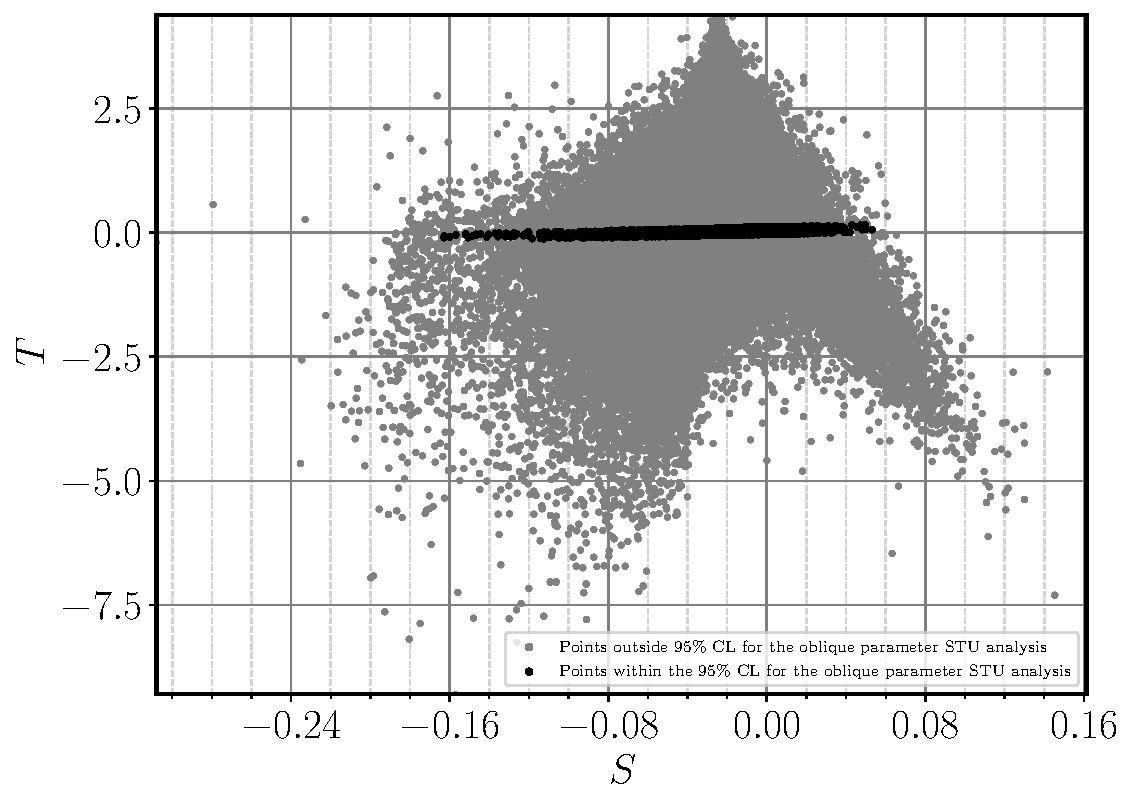
\includegraphics[width=.49\textwidth]{Images/3HDM/EW/EW_S_T_black.pdf}	
	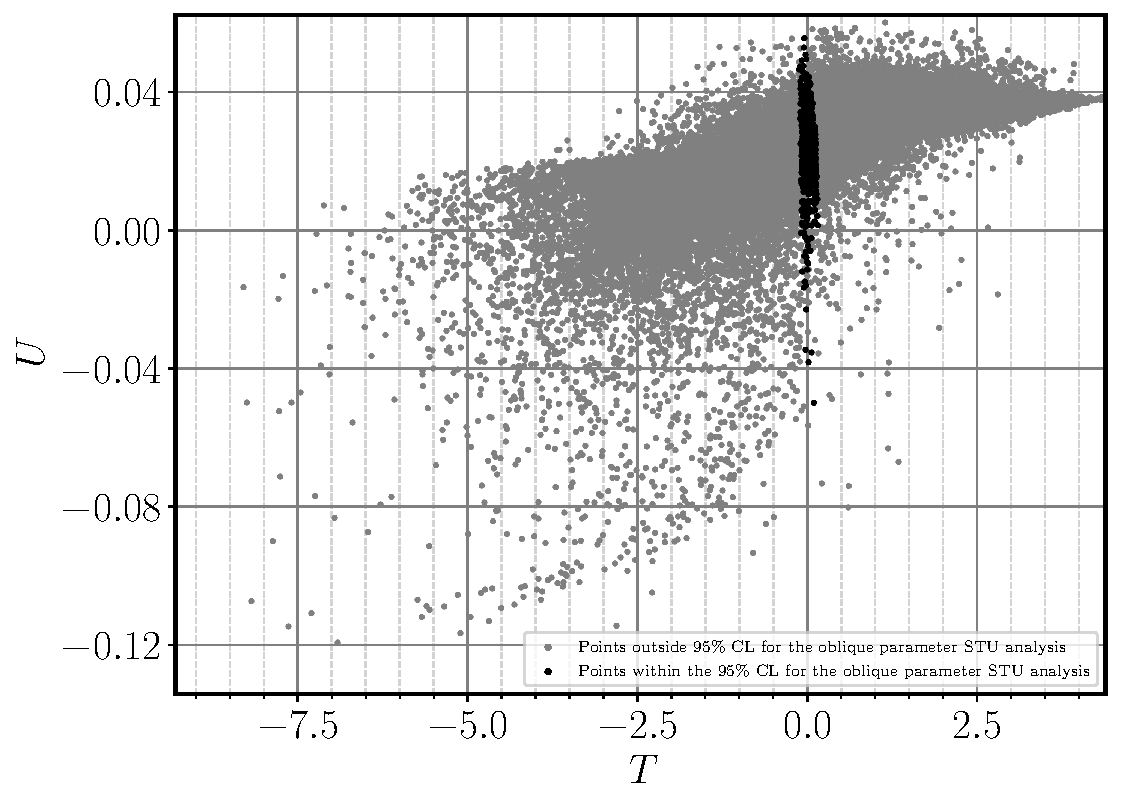
\includegraphics[width=.49\textwidth]{Images/3HDM/EW/EW_T_U_black.pdf}
	\caption{3HDM scatter plots for EW  precision  observables  showing  the ST(left)  and TU(right)planes.  Accepted points lying within a 95\% C.L. ellipsoid of the best fit point are represented inblack whereas grey points are excluded.}
	\label{Fig:3HDM_STU}
\end{figure}
%
We can clearly see that NP can have a very strong effect on some of these observables, most notably in the deviation in the T variable.
%
Note that this wide variation makes the elipsoid seen previously look like a narrow region. 
%
As in the B-L-SM the values for $(\Delta S , \Delta T , \Delta U )$ are taken from \cite{Baak_2012}.

% Meantion :  In order to test the obliqueparameters, we implement results for the SM fit from the Gfitter collaboration [45].   %  M. Baak, M. Goebel, J. Haller, A. Hoecker, D. Ludwig, K. Moenig et al.,UpdatedStatus of the Global Electroweak Fit and Constraints on New Physics,Eur. Phys. J.C72(2012) 2003 [1107.0975] 

\subsubsection{Higgs Constraints}

The STU results discussed we can continue our work by showing the available corresponding physical parameter space. 
%
Recall that our inversion process logarithmic scanned over the 16 real parameters in this space, the scalar masses, soft breaking terms and all mixing angles.  
%
%For brevity we will present our results only in order to the scalar masses,
%We can begin by observing the available scalar space. 
%
%Let us describe regions for masses and VEVs that are allowed by Higgs data constraints and EW precision tests. 

It is important to mention that the labeling of the scalars is arbitrary, we just ensure that the scalars are labeled in growing mass order e.g. $m_{H^\pm_2} > m_{H^\pm_1}$. 
%
This change does not have any real physical significance but it leaves our graphs with a linear cut where $m_i = m_j$. 
%
\begin{figure}[H]
	\centering
	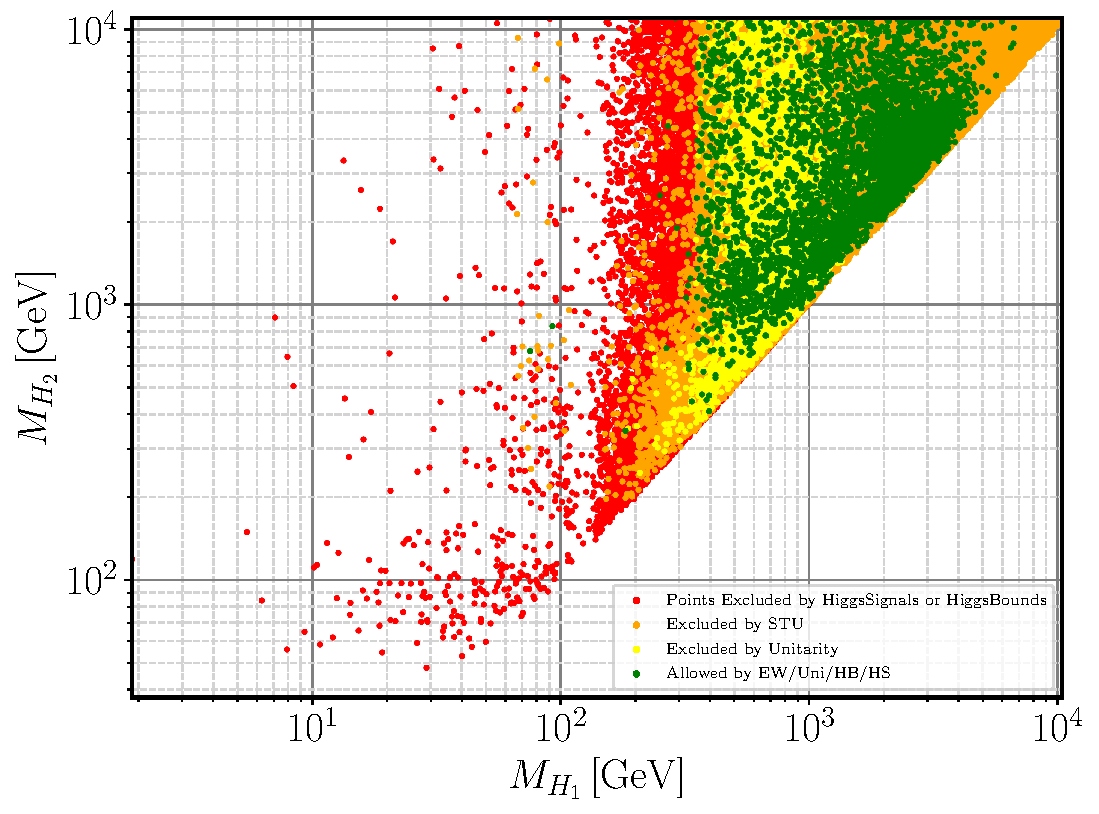
\includegraphics[width=.49\textwidth]{/3HDM/H1_H2.pdf}
	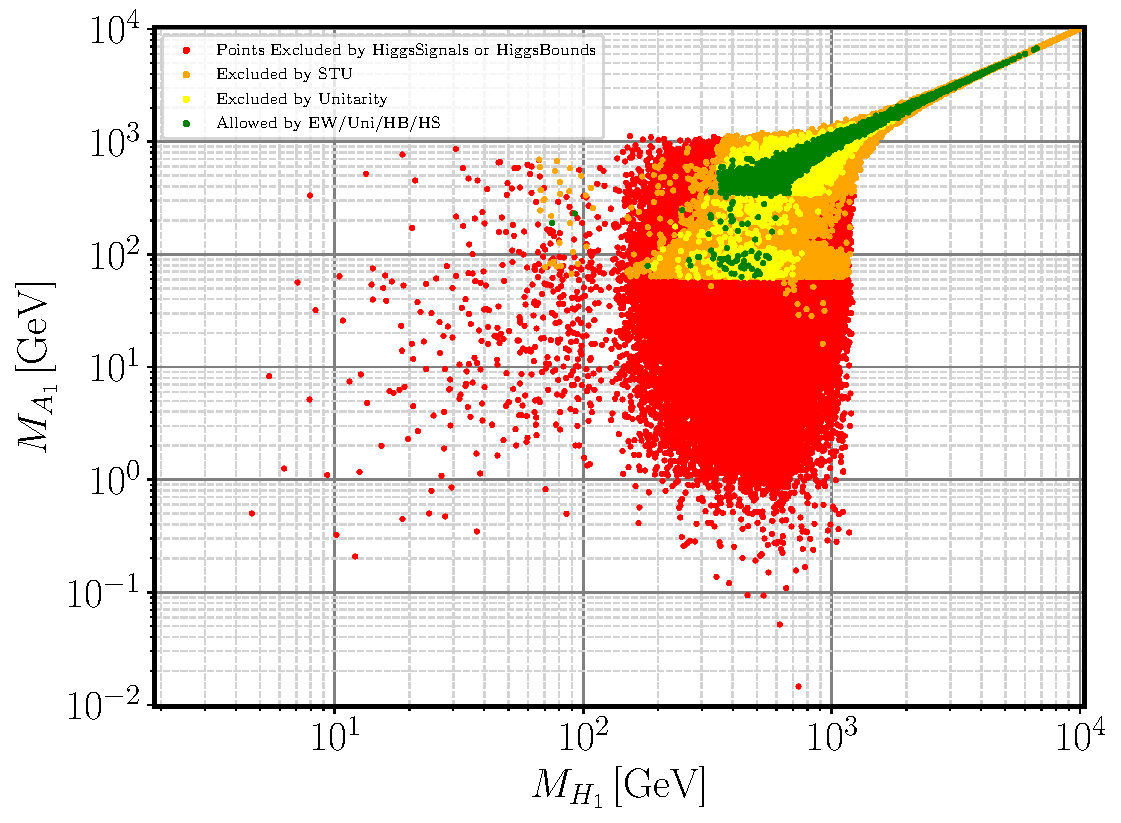
\includegraphics[width=.49\textwidth]{/3HDM/H1_A1.pdf}
\end{figure}	
\begin{figure}[H]\ContinuedFloat
    \centering
	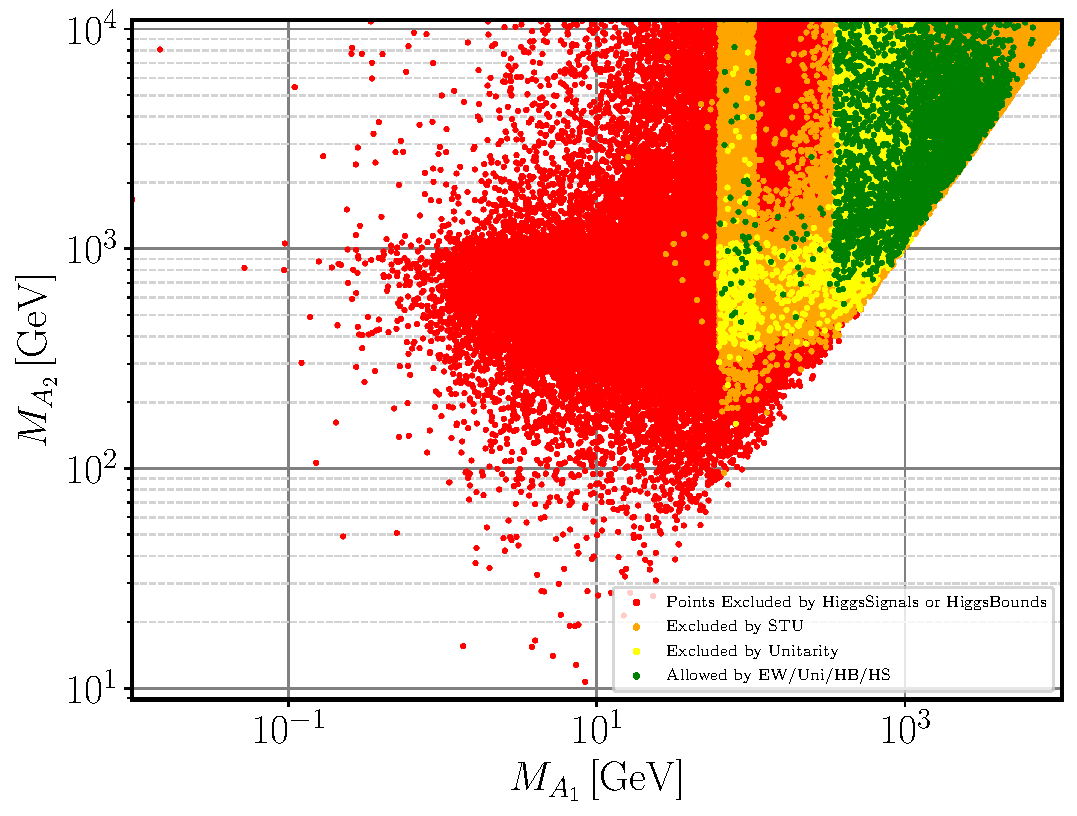
\includegraphics[width=.49\textwidth]{/3HDM/A1_A2.pdf}
	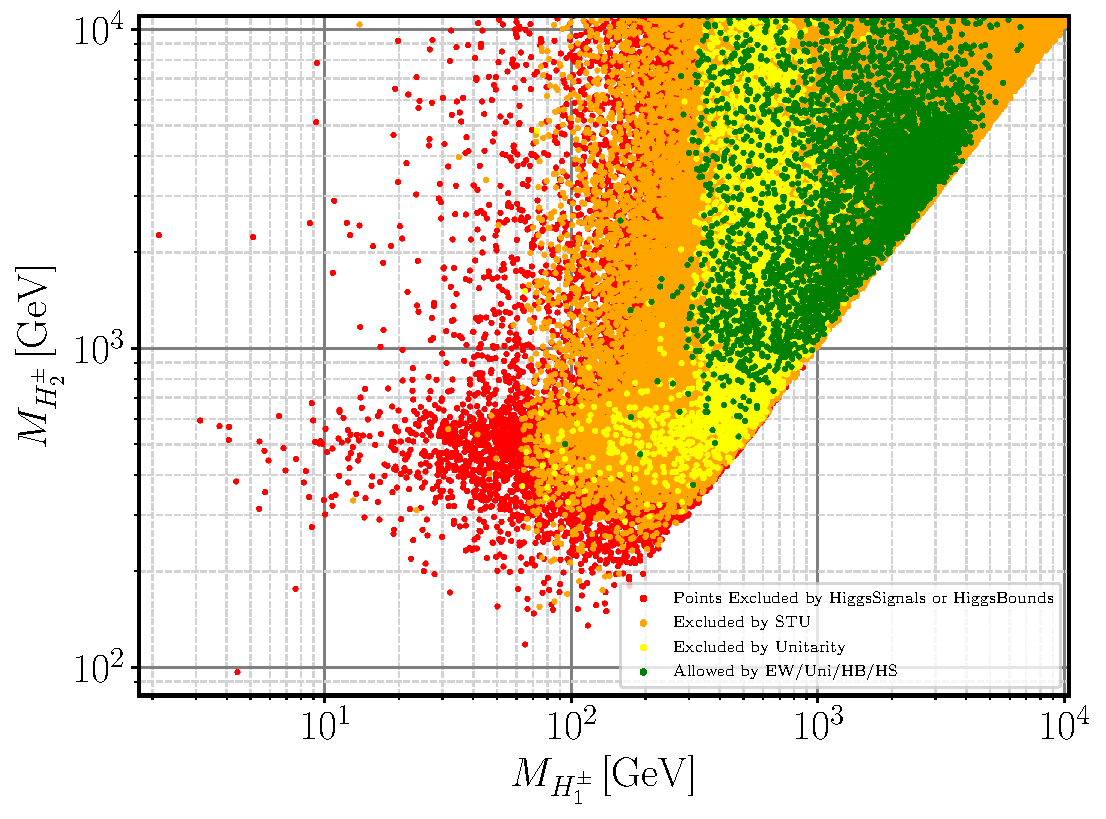
\includegraphics[width=.49\textwidth]{/3HDM/Hc1_Hc2.pdf}
	\caption{Scatter plots of parameter space allowed under several cuts imposed on the BGL-like 3HDM. On the upper right side we have the plot showing the masses of the two heavier CP-even scalars $H_2$ and $H_1$ while in the right we show the relation between the lightest (non SM Higgs) of the CP-even and pseudoscalar particles. As for the bottom plots see the remaining CP-odd scalars and how they are excluded under several cuts. Right we have the pseudoscalar masses $A_1$ and $A_2$ while in the left side we have the CP- odd charged Higgs states $H_1^\pm$ and $H_2^\pm$.	Red points failed HS and HB tests; yellow points violate unitarity constraints; orange points only fail electroweak precision constraints, and green ones satisfy all restrictions.}
	\label{fig:H1_A1_Plots}
\end{figure}	

%One important characteristic of our results worth discussing is the presence of relatively light  scalars. 
%
We can observe that direct searches tightly constrain the pseudoscalar and scalar masses. 
%
These direct search exclusions are directly tied to the red zones where HiggsBounds and HiggsSignals do not allow scalars to exist. 
%
Further examination of these areas shows, firstly the lighter values for the pseudoscalar masses are all excluded by direct Higgs. However there is space for pseudoscalars in case they are "masked" by the observed SM-like Higgs boson signal.  
%
As for all other scalars there does not seem to be a way to reproduce the same effect. 

Furthermore, observing the top right figure in Fig\,\ref{fig:H1_A1_Plots}, direct searches are not responsible for the exclusion of lighter charged Higgs, but our model can not respect STU limits and unitarity constraints for ligther charged Higgs.  

%Next there is a zone within where STU limits are fulfilled at 95 \% C.L. and within that zone we see that only a small region respects unitarity constraints. 
%
We can then argue that our model should predict the existence of masses as low as a few hundred GeVs motivating the continuation of direct searches at the LHC. 
%
The precise values for benchmark points will be presented after the Quark flavour observables are performed. 

%{ \color{red} Ask morais : why do pseudo scalar masses tend to funnel? }  

%We can then argue that our model predicts the existence of masses around (300's GeVs check in detail later) which are in harmony with the SM i.e. are so far compatible with observations. 

A feature of HiggsBounds is it also enables us to see the most stringent channel for a given parameter point. 
%
From this we can see the most stringent channels that constrict our model are di-photon production and gluon fusion into light scalars (Limits taken from Refs. \cite{Aad_2014,CMS-PAS-HIG-14-029,Khachatryan_2015}). 
%
%It could be that by requiring that we have a SM-like Higgs boson, naturally imposes conditions upon the couplings of the heavier (or lighter) CP-even scalar states to the Gauge bosons. This should enable most of the Higgs sector to be within bounds. 
%
%, and seeing that the harshest condition on most scalar sectors is the di-Z production we then have that due to the alignment limit imposed the majority of the scalar sector is allowed. 
%
%We can also see that unless the signal coming from the pseudoscalar masses is masked by the Higgs SM signal or the pseudoscalar is heavy (in the TeV region) that it poses a harsh cut on the parameter space.

%{ \color{red} Why then are the pseudoscalars so constricted. }   

\subsubsection{Flavour Cuts }

% Having shown that there are no instances of heavy fine tuning in our model. 

Let us now look at the QFV observable results, first by constraining all the most stringent QFV to be within 2 $\sigma$ bounds as discussed previously,
%
% Before showing what combined regions we observe stemming from the cuts discussed above when combined with QFV observables, it might be a worth while endevour to see what type of regions we can see with only QFV observables. 
%
%First we show what the fractions of QFV observables show,    
%
%\begin{figure}[H]
%	\centering
%	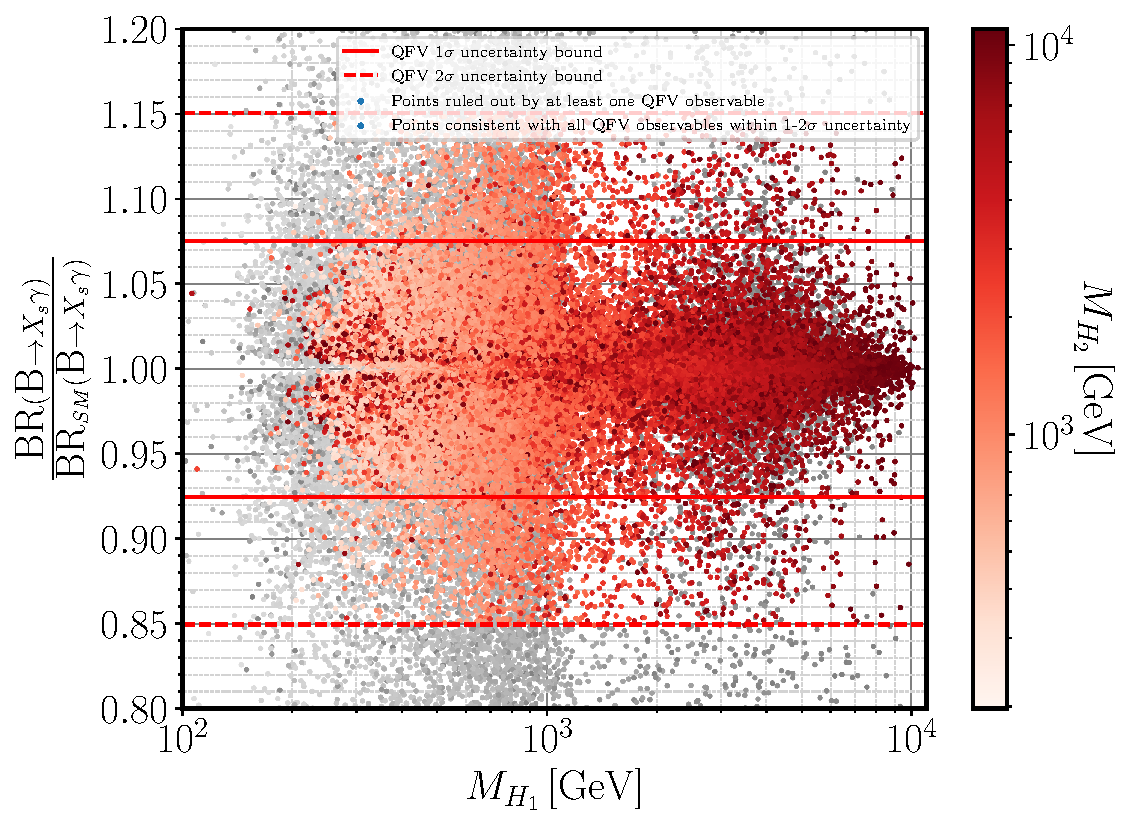
\includegraphics[width=.49\textwidth]{Images/3HDM/Reds/Xsgamma_H1_H2.pdf}
%	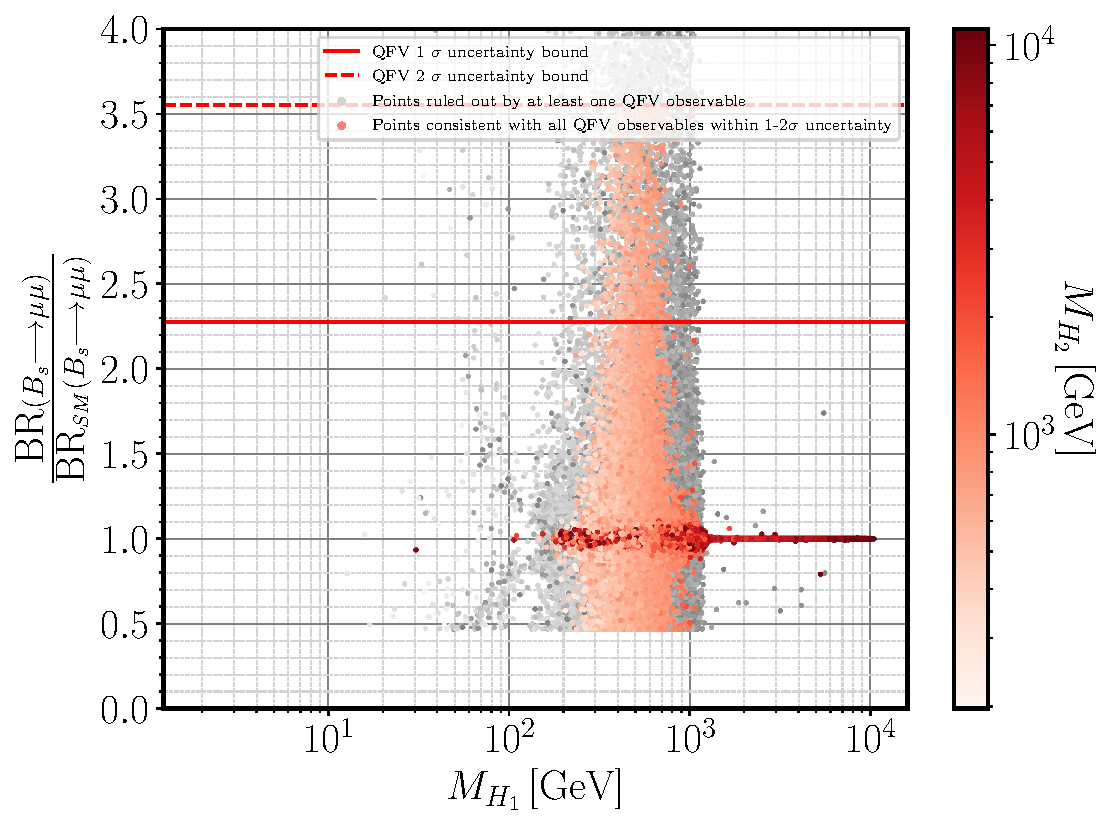
\includegraphics[width=.49\textwidth]{Images/3HDM/Reds/Bsmumu_H1_H2.pdf}
%\end{figure}
%\begin{figure}[H]\ContinuedFloat
%    \centering
%	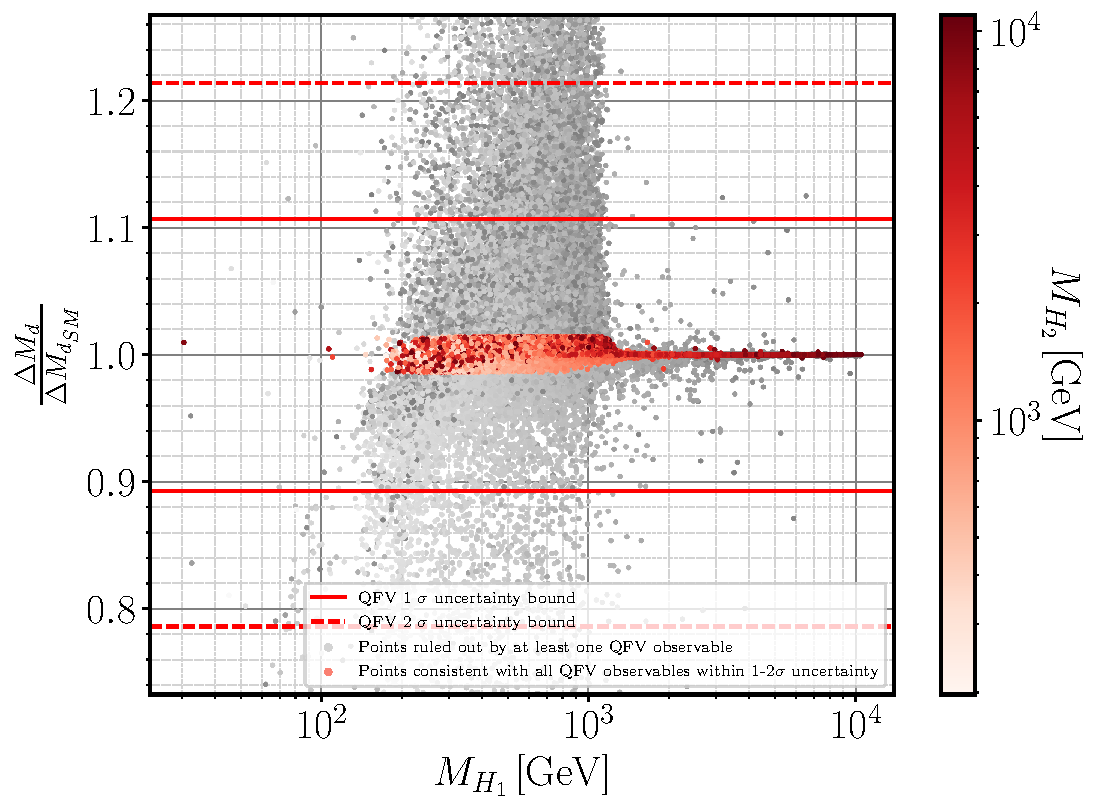
\includegraphics[width=.49\textwidth]{Images/3HDM/Reds/DeltaMd_H1_H2.pdf}
%    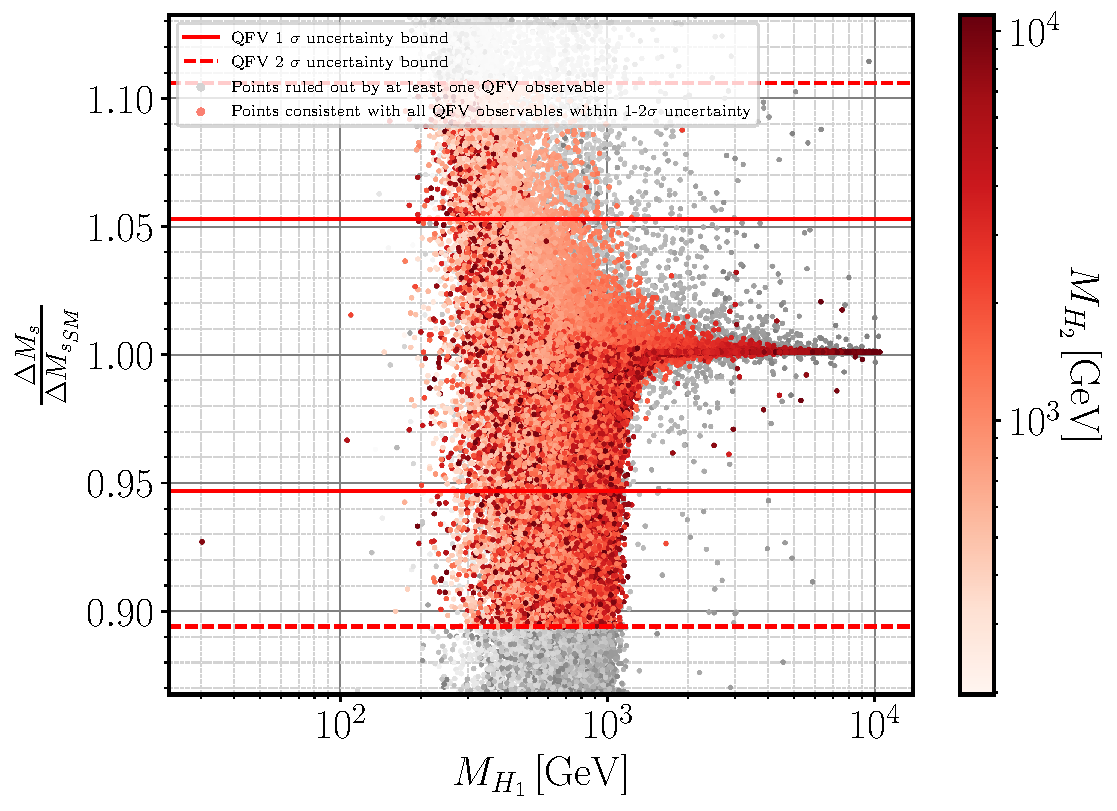
\includegraphics[width=.49\textwidth]{Images/3HDM/Reds/DeltaMs_H1_H2.pdf}
%\end{figure}
%\begin{figure}[H]\ContinuedFloat
%    \centering
%    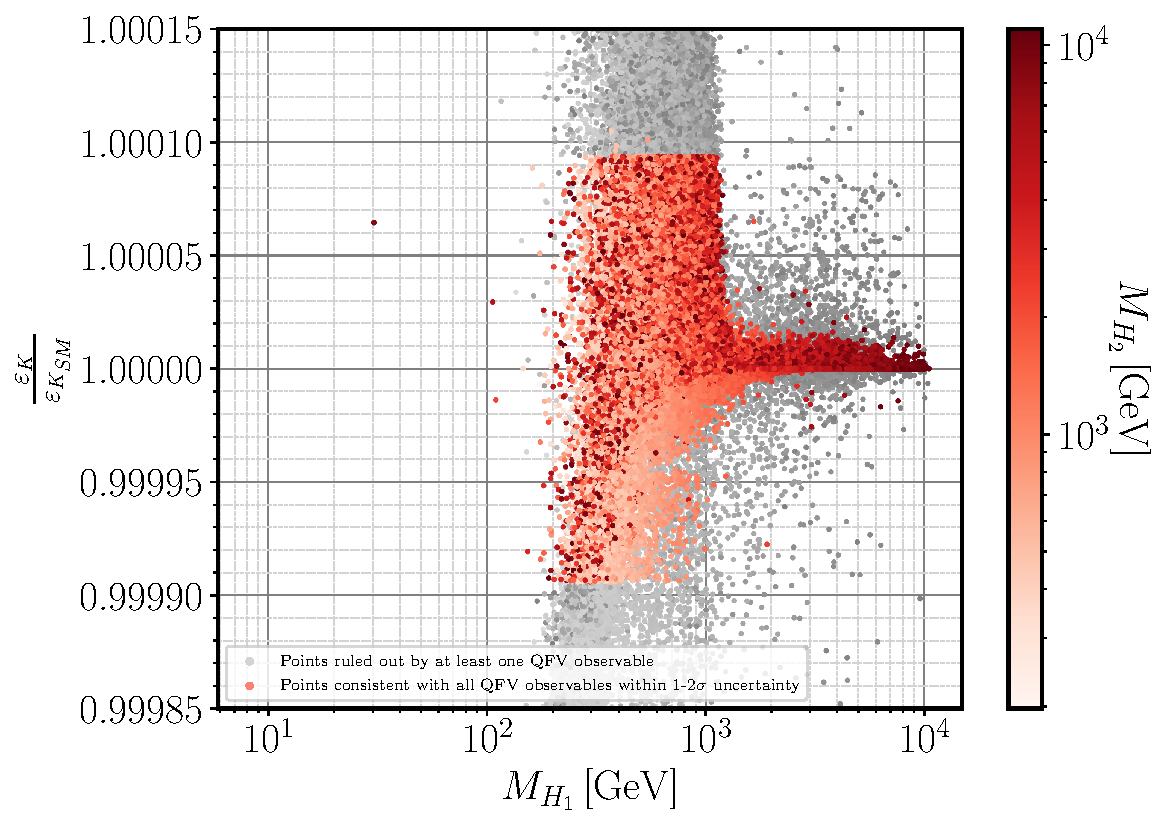
\includegraphics[width=.49\textwidth]{Images/3HDM/Reds/Eps_K_H1_H2_Centered.pdf}
%	\caption{ Scatter plot of the estimated QFV observables normalized to the SM values versus the lightest scalar Higgs. The grey points in all plots represent a point that would be outside the 2 $\sigma$ bound for one of the observables while in a red color scale we see the second CP-even neutral scalar mass for the remaining points. % {\color{blue} Ask, anyone of these are $H^\pm$ only? is it worth swapping H?}  
%	}
%	\label{fig:3HDM_Flavour}
%\end{figure}

\begin{figure}[H]
\centering
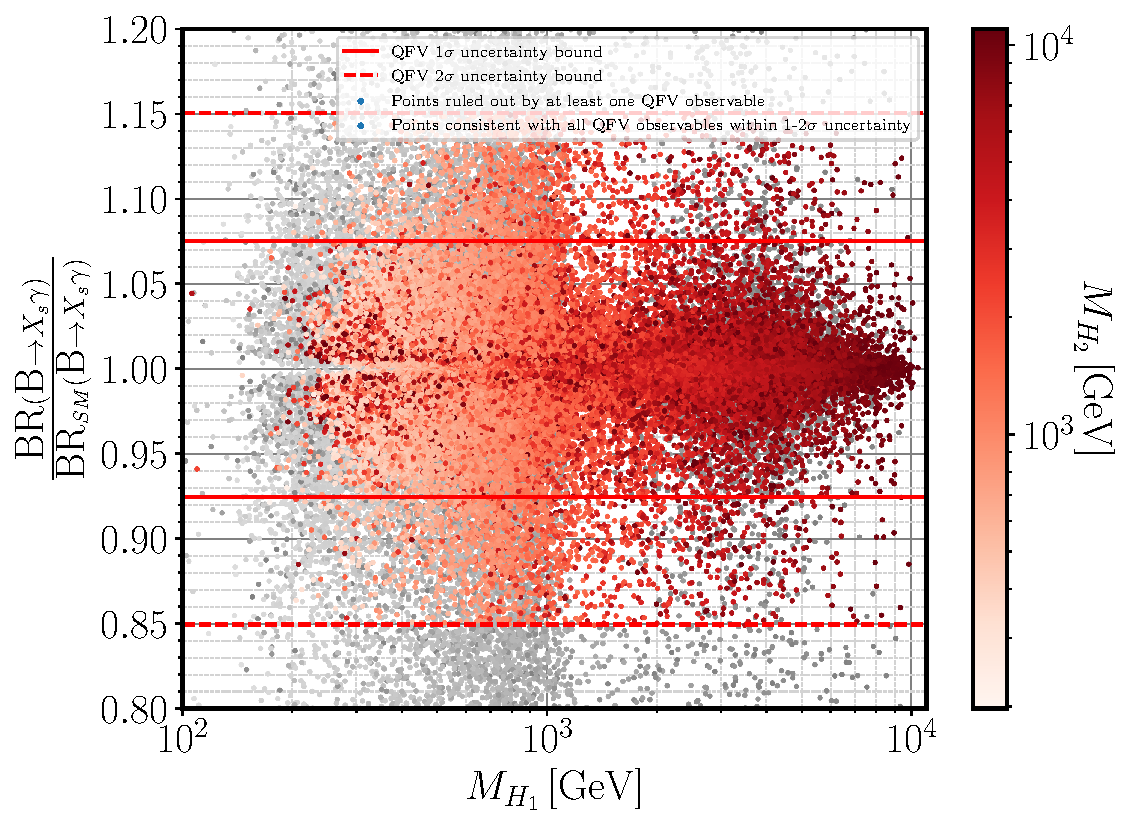
\includegraphics[width=.49\textwidth]{Images/3HDM/Reds/Xsgamma_H1_H2.pdf}
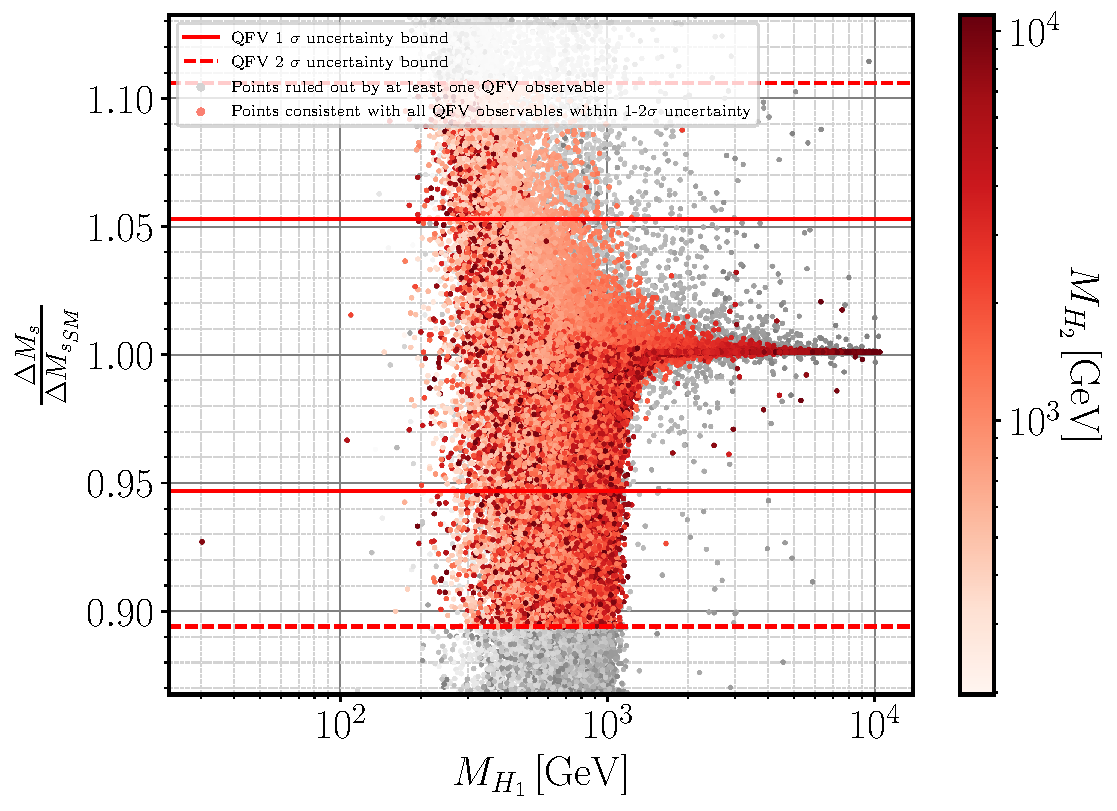
\includegraphics[width=.49\textwidth]{Images/3HDM/Reds/DeltaMs_H1_H2.pdf}
%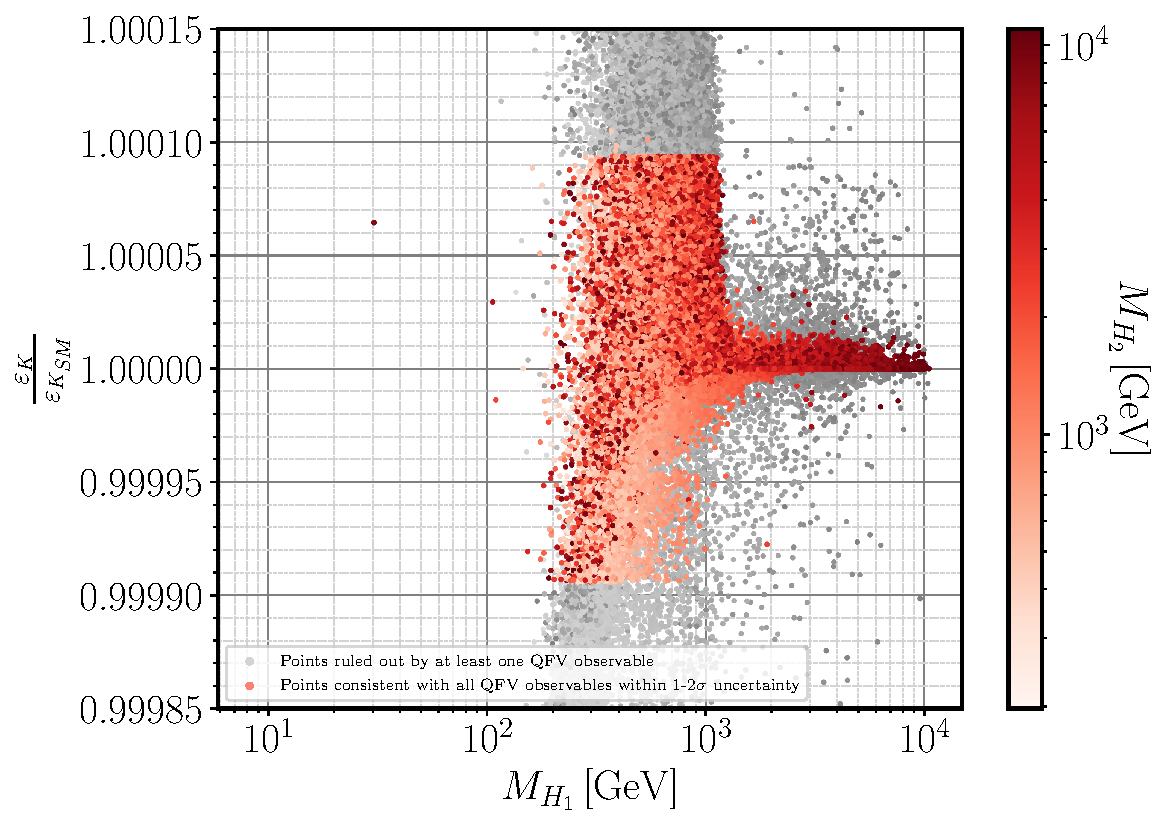
\includegraphics[width=.49\textwidth]{Images/3HDM/Reds/Eps_K_H1_H2_Centered.pdf}
	\caption{ Scatter plot of the estimated QFV observables normalized to the SM values versus the lightest scalar Higgs. The grey points in all plots represent a point that would be outside the 2 $\sigma$ bound for one of the observables while in a red color scale we see the second CP-even neutral scalar mass for the remaining points. % {\color{blue} Ask, anyone of these are $H^\pm$ only? is it worth swapping H?}  
	}
	\label{fig:3HDM_Flavour}
\end{figure}

%The bounds shown in these Figures are seen in, 

%\begin{table}[H]
%\centering
%\begin{tabular}{|l|c|c|c|c|c|c} 
%\hline
%                           & $\dfrac{\textrm{BR} ( \textrm{B} \rightarrow X_s \gamma)}{\textrm{BR}_{SM} ( \textrm{B} \rightarrow X_s \gamma )}$ &  $\dfrac{ \textrm{BR} (B_s  \longrightarrow  \mu  \mu )}{\textrm{BR}_{SM}(B_s  \longrightarrow  \mu  \mu ) }$  
%                           & $\dfrac{\Delta M_d}{\Delta M_{d_{SM}} }$ 
%                           & $\dfrac{\Delta M_s}{\Delta M_{s_{SM}} }$
%                           & $\dfrac{\varepsilon_K}{\varepsilon_{K_{SM}}}$   \\ \hline 
%$1 \sigma$ upper QFV bound &  1.08    &  2.27   &  1.10     &  1.05     &    1.13    \\ \hline 
%$1 \sigma$ lower QFV bound &  0.91    &  0.00   &  0.91     &  0.95     &    0.87    \\ \hline 
%$2 \sigma$ upper QFV bound &  1.15    &  3.55   &  1.21     &  1.10     &    1.27    \\ \hline 
%$2 \sigma$ lower QFV bound &  0.85    &  0.00   &  0.79     &  0.90     &    0.72    \\ \hline  
%\end{tabular}
%\caption{Calculated 1 and 2 $\sigma$ bounds for QFV observables}
%\end{table}

Note the available zone for $\varepsilon_K/\varepsilon_{K_{SM}}$ and some other decays seems quite small, this is due to ${\textrm{BR} ( \textrm{B} \rightarrow X_s \gamma)}/{\textrm{BR}_{SM} ( \textrm{B} \rightarrow X_s \gamma )}$ and ${\Delta M_s}/{\Delta M_{s_{SM}} }$ being very tightly constraint and the most sensitive in our model.

When combined with the EW and scalar analysis these exclusions wield, 

\begin{figure}[H]
	\centering
	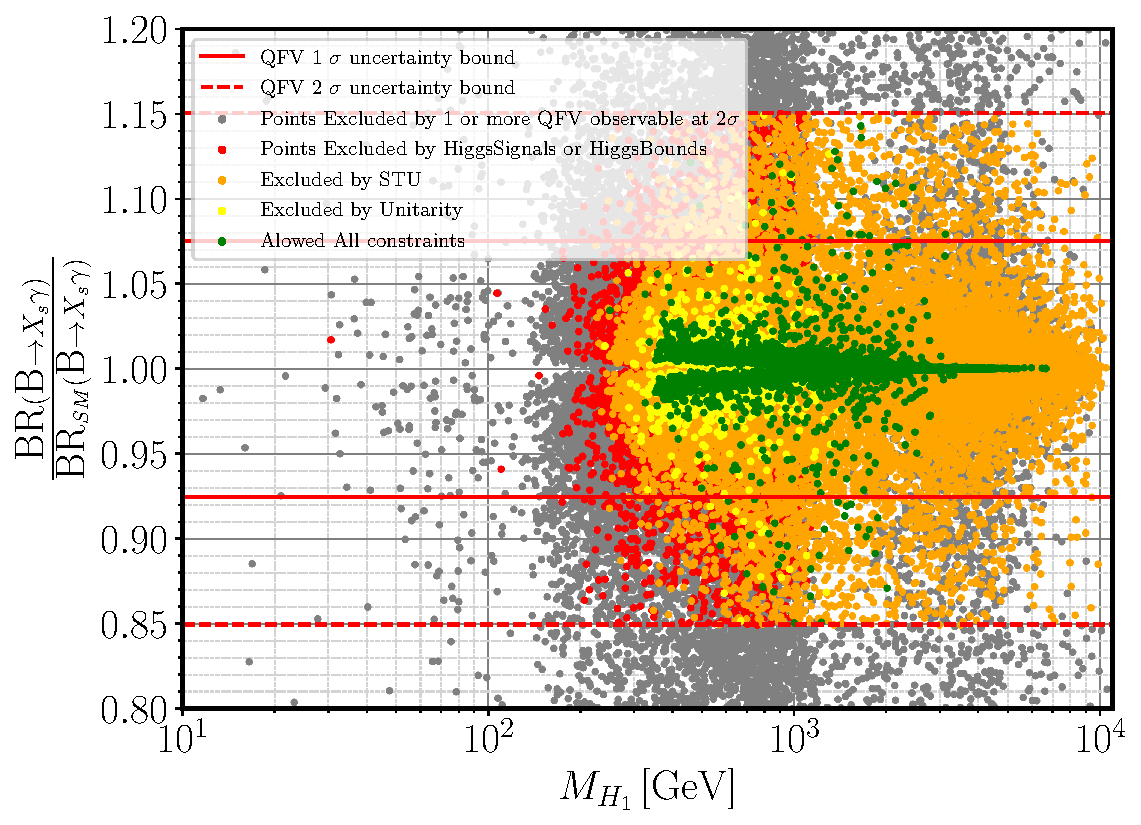
\includegraphics[width=.49\textwidth]{Images/3HDM/PT_Folder/XsGamma_H1.pdf}
	%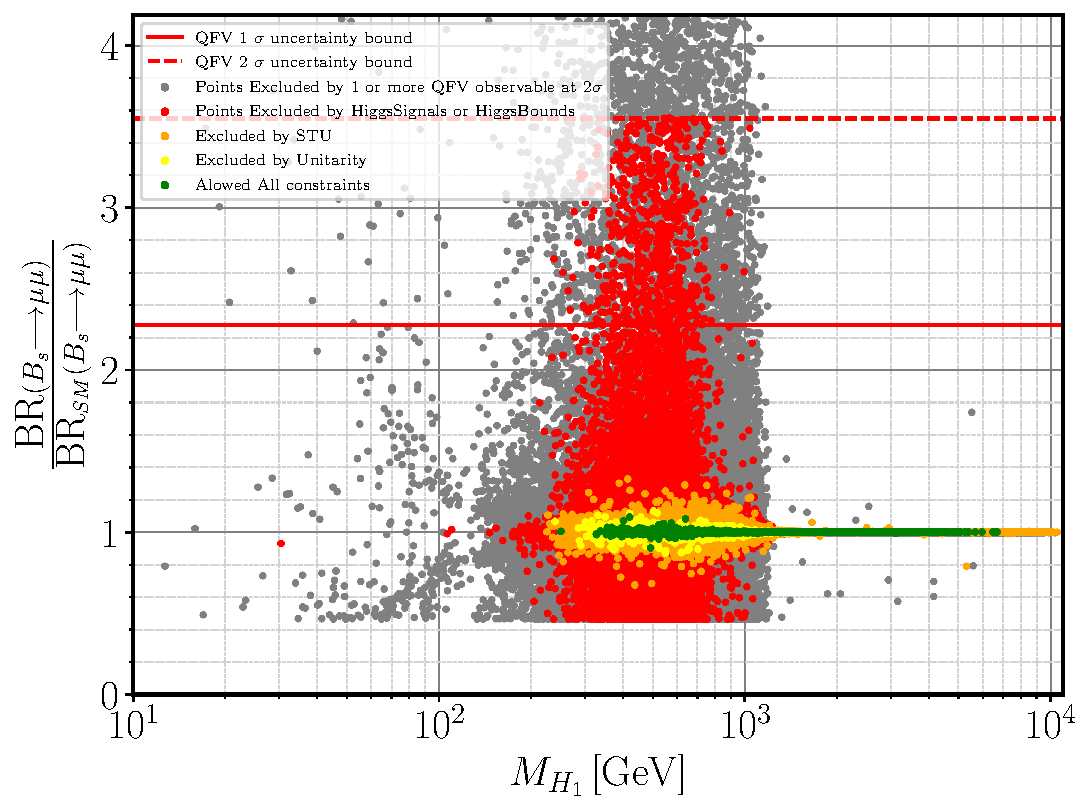
\includegraphics[width=.49\textwidth]{Images/3HDM/PT_Folder/Bsmumu_H1.pdf}
    %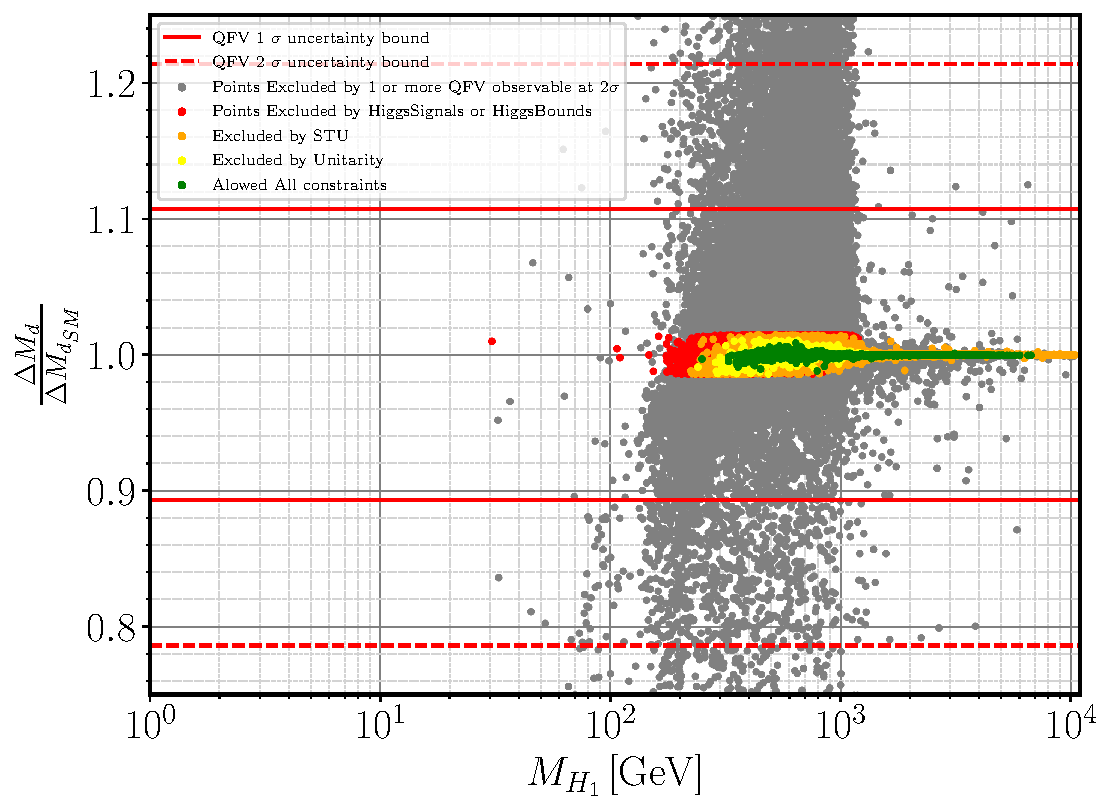
\includegraphics[width=.49\textwidth]{Images/3HDM/PT_Folder/Delta_Md_H1.pdf}
    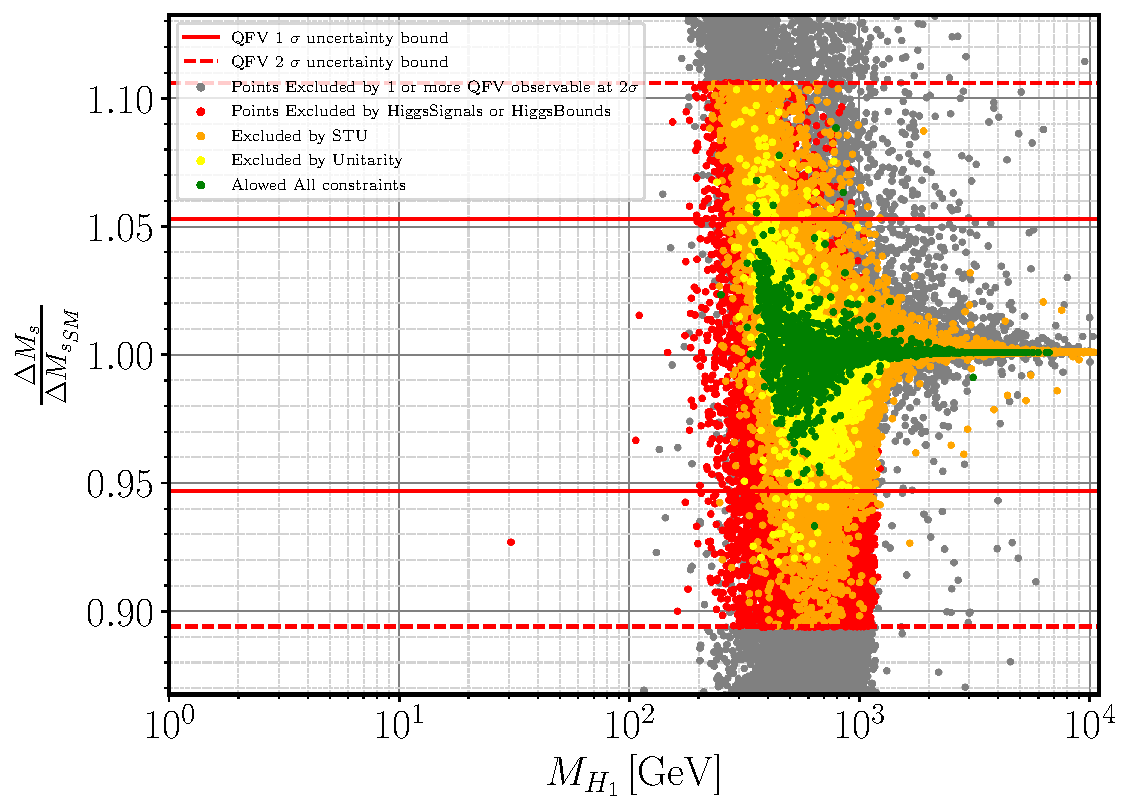
\includegraphics[width=.49\textwidth]{Images/3HDM/PT_Folder/Delta_Ms_H1.pdf}
    %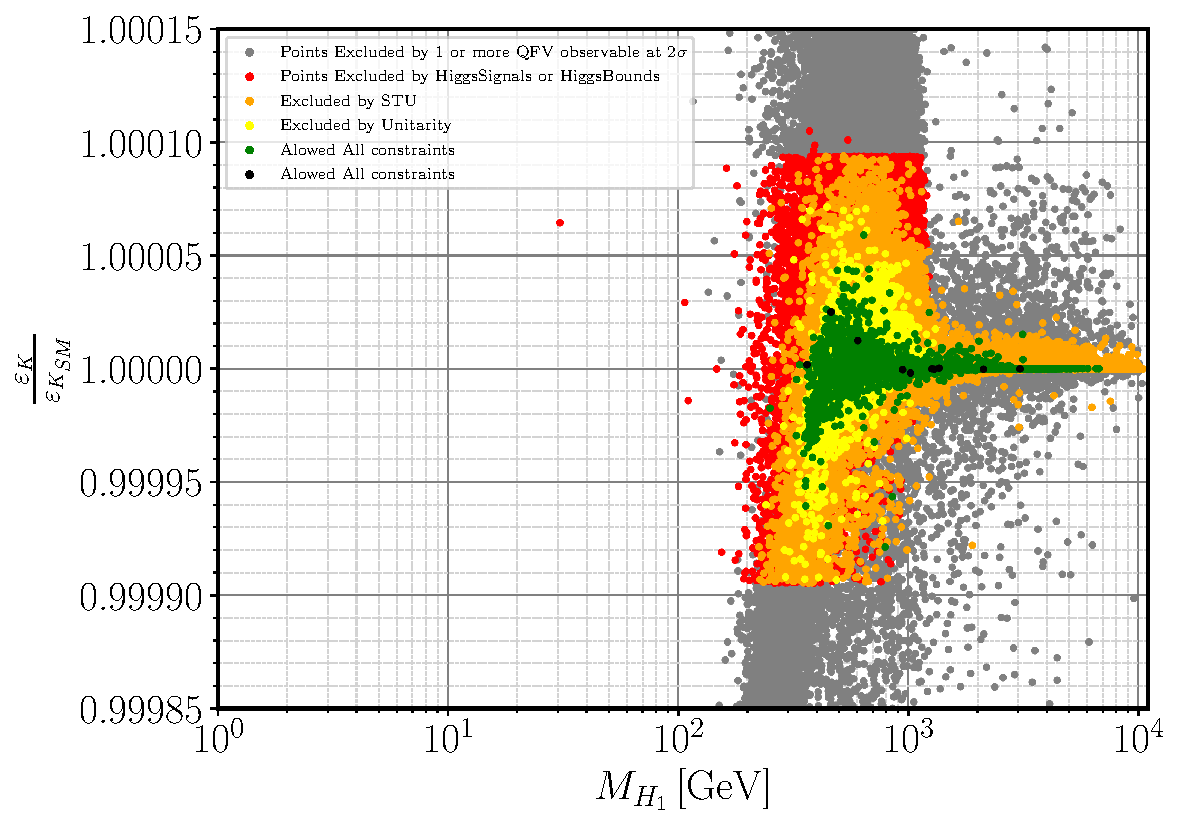
\includegraphics[width=.49\textwidth]{Images/3HDM/PT_Folder/Eps_K_H1_Thighter_Centered.pdf}
    \caption{ Scatter plot of the estimated QFV observables normalized to SM values overlaped with EW and Higgs sector just as in previous figures. } 
	\label{fig:3HDM_Flavour_PT}
\end{figure}	

Here you can clearly see that there is a central region where the points that verify all EW and scalar constraints are all also consistent with QFV observables. 
%
This is a very important conclusion we take from our model. Trough the stabilization of the 3HDM by the flavour symmetry all QFV observables are kept under significant deviation for all the viable mass spectrum.  

We can now extract possible bench mark points, these are written in Tab.\,\ref{Tab:BadTable}.
%
%\begin{table}[H]
%\label{tab:3HDM-Benchmarks-Mass}
%\centering
%\begin{tabular}{l|c|c|c|c|c|c|}
%\cline{2-7}
%                                                  & $H_1$ & $H_2$ & $A_1$ & $A_2$ & $H_1^\pm$ & $H_2^\pm$ \\ \hline
%\multicolumn{1}{|l|}{$\text{Max}_M \ (\text{GeV})$} & 6664  & 10979 & 6683  & 10995 & 6623      & 10989     \\ \hline
%\multicolumn{1}{|l|}{$\text{Min}_M \ (\text{GeV})$}              & 251   & 412   & 87    & 395   & 157       & 374       \\ \hline
%\end{tabular}
%\caption{Possible new discovery points, lightest set of scalars that survive all constraints.}
%\end{table}

%\begin{table}[!htb]
%\centering
%\begin{tabular}{|c|c|c|c|c|c|c|}
%\hline
%                          & $m_{H_1}$ (GeV) & $m_{H_2}$ (Gev) & $m_{A_1}$  (GeV) & $m_{A_2}$  (GeV) & $m_{H^\pm_1}$  (GeV) & $m_{H^\pm_2}$  (GeV) \\ \hline
%Lightest $H_1$            & 251 & 2488 & 247 & 2616 & 157 & 2510    \\ \hline
%Second lightest $H_1$     & 327 & 1528 & 359 & 1616 & 229 & 1561    \\ \hline
%Lightest $A_1$            & 386 & 452  & 87  & 467 & 189  & 466      \\ \hline
%Second lightest $A_1$     & 337 & 446  & 100 & 395 & 311  & 374      \\ \hline
%Lightest $H^\pm_1$        & 251 & 2488 & 247 & 2616 & 157 & 2510   \\ \hline
%Second lightest $H^\pm_1$ & 398 & 1314 & 282 & 1525 & 173 & 1314
%
%      \\ \hline
%\end{tabular}
%\end{table}

%
\begin{table}[H]
\centering
\begin{tabular}{c|c|c|c|c|c|c|}
\cline{2-7} 
                                                          & $m_{H_1}$ & $m_{H_2}$ & $m_{A_1}$ & $m_{A_2}$ & $m_{H^\pm_1}$ & $m_{H^\pm_2}$ \\ \hline
\multicolumn{1}{|c|}{\multirow{2}{*}{Lightest $H_1$}}     & 251 & 2488 & 247 & 2616 & 157 & 2510  \\ \cline{2-7} 
\multicolumn{1}{|c|}{}                                    & 327 & 1528 & 359 & 1616 & 229 & 1561  \\ \hline
\multicolumn{1}{|c|}{\multirow{2}{*}{Lightest $A_1$}}     & 386 & 452  & 87  & 467 & 189  & 466  \\ \cline{2-7} 
\multicolumn{1}{|c|}{}                                    & 337 & 446  & 100 & 395 & 311  & 374  \\ \hline
\multicolumn{1}{|c|}{\multirow{2}{*}{Lightest $H^\pm_1$}} & 251 & 2488 & 247 & 2616 & 157 & 2510 \\ \cline{2-7} 
\multicolumn{1}{|c|}{}                                    & 398 & 1314 & 282 & 1525 & 173 & 1314 \\ \hline
\end{tabular}
\caption{A selection of four benchmark points. All written masses are given in GeV. These correspond to the lightest scalars found that respect all QFV and scalar sector cosntraints.}
\end{table}

We discussed that some NHDMs use deliberate fine-tuning in their model as to have NP contributions balance out and artificially control flavour changing effects in their models. In this model we do not follow this process, our scans were purely randomly generated.  
%
However, randomness combined with thew large amount of data collected could have found a syncronicity where flavour observables are fine-tunned by accident. 
%
%It was important to verify fine-tunning as our scans randomness could have found a syncronicity where flavour observables are fine-tunned by accident. 

To check if this phenomena was present, all points were recalculated with slight a variation of masses trough a 1\% variation of soft breaking terms, $\mu_{13}$, $\mu_{23}$ and $\mu_{21}$. 
%
Such a mass variation is expected to lead to variation of the flavour channel decay amplitude. 

Trough this exercise we expect to show that a there is no abruptly high variation of masses or QFV observable as to show no fine-tunning is present.
% 
The results can be seen in, 

\begin{figure}[H]
	\centering
	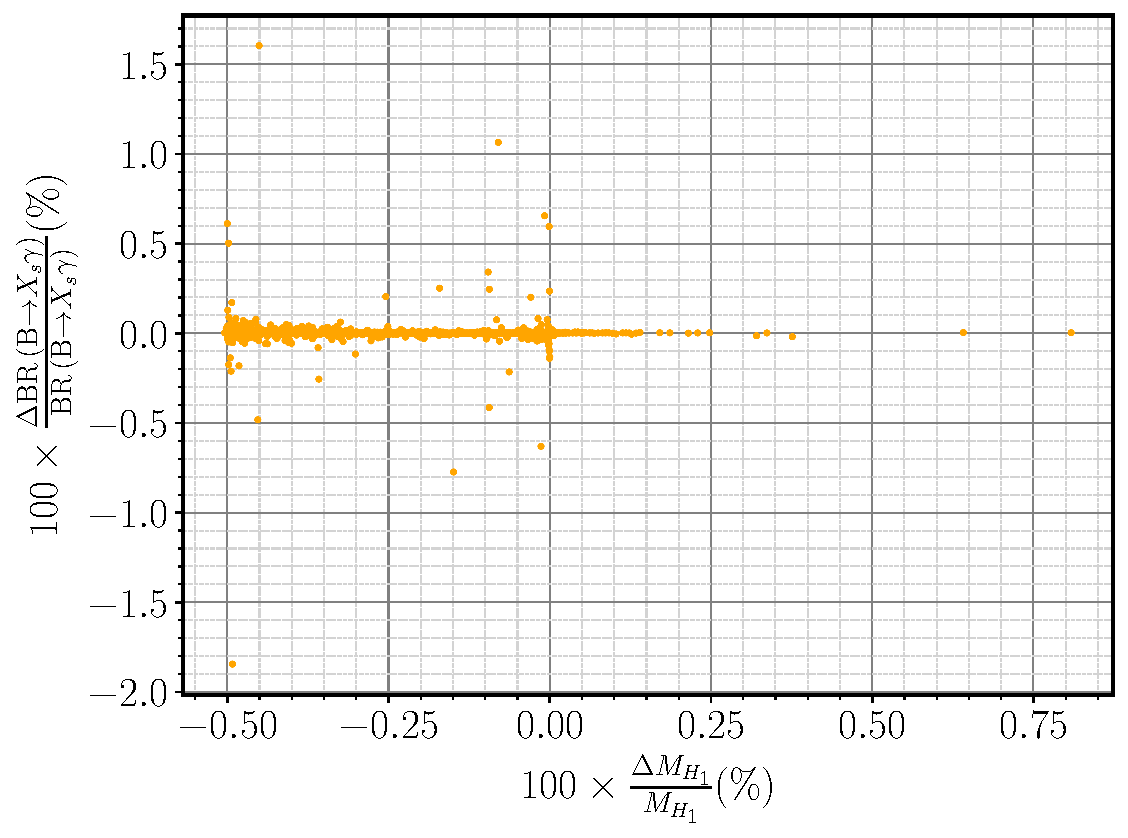
\includegraphics[width=.49\textwidth]{Images/3HDM/Fine_Tuning/Xsgamma_H1.pdf}
	%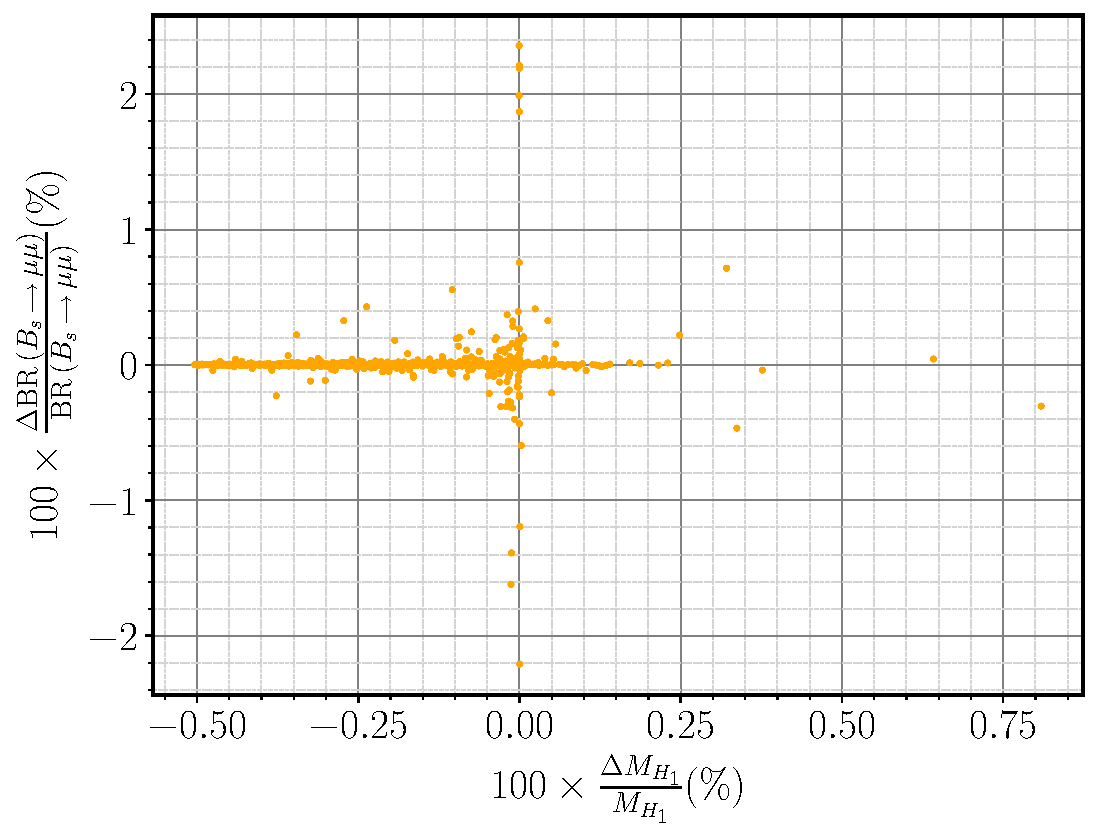
\includegraphics[width=.49\textwidth]{Images/3HDM/Fine_Tuning/Bsmumu_H1.pdf}
	%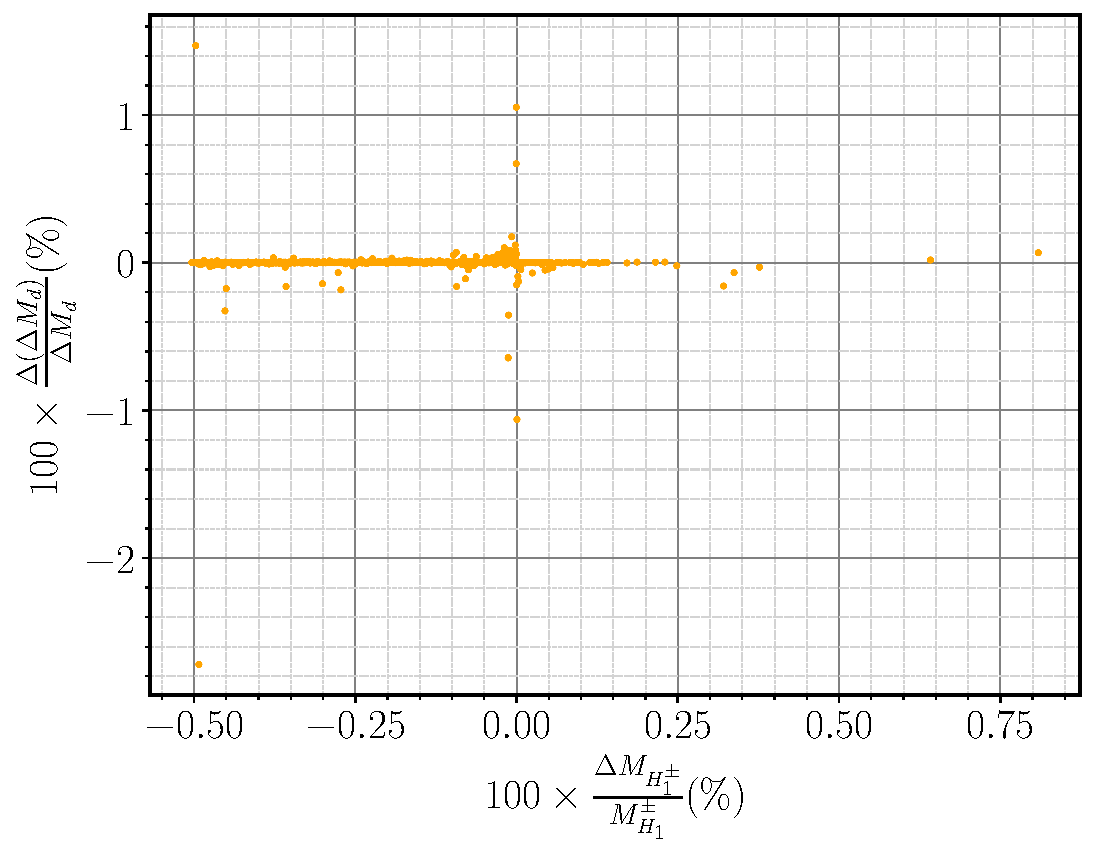
\includegraphics[width=.49\textwidth]{Images/3HDM/Fine_Tuning/DeltaMd_H1.pdf}
    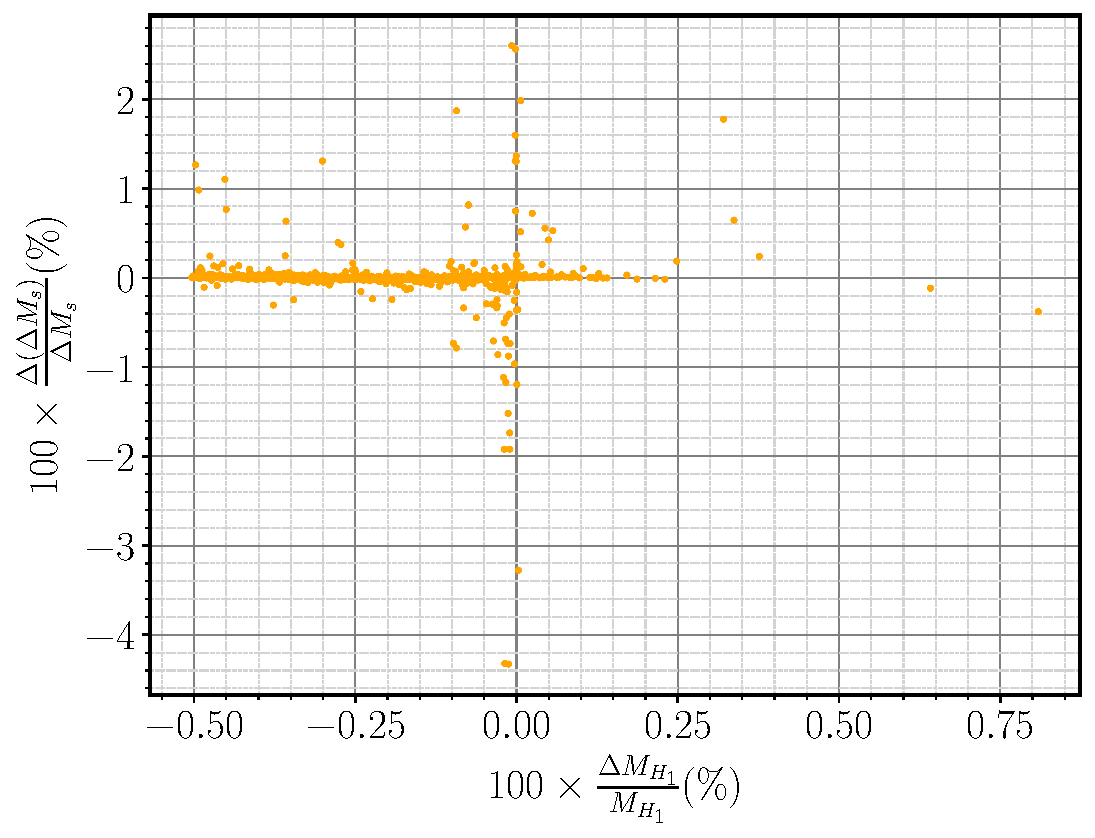
\includegraphics[width=.49\textwidth]{Images/3HDM/Fine_Tuning/DeltaMs_H1.pdf}
    %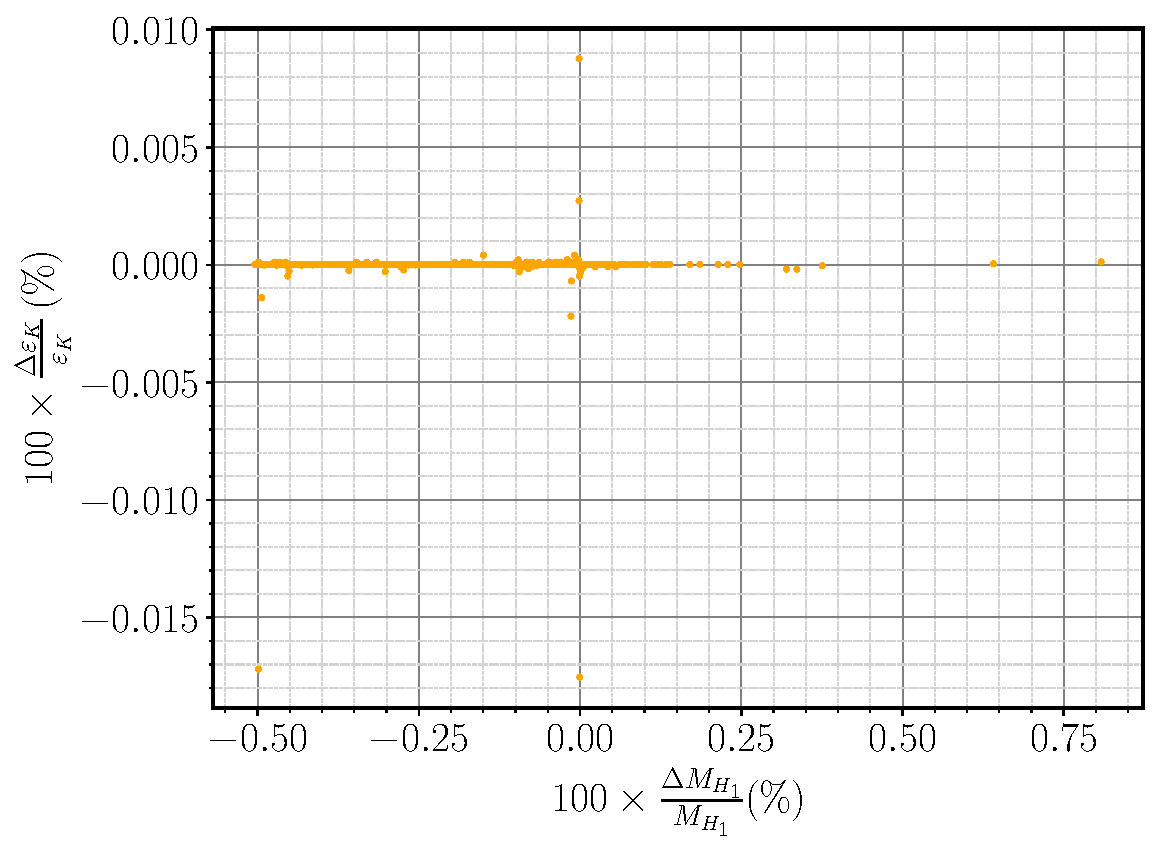
\includegraphics[width=.49\textwidth]{Images/3HDM/Fine_Tuning/eps_K_H1.pdf}
	\caption{Relative mass and QFV observable changes with the increase of 1\% in all softbreaking terms}
	\label{fig:3HDM_Fine_Tunning}
\end{figure}	

Finally a complementary study was also implemented trough Madgraph in this model. 
%
This study served a dual purpose to ensure that proper gluon fusion was being calculated by HiggsBounds and HiggsSignals and to show how close the model was to exclusion. The results are seen in, 
%
\begin{figure}[H]
	\centering
	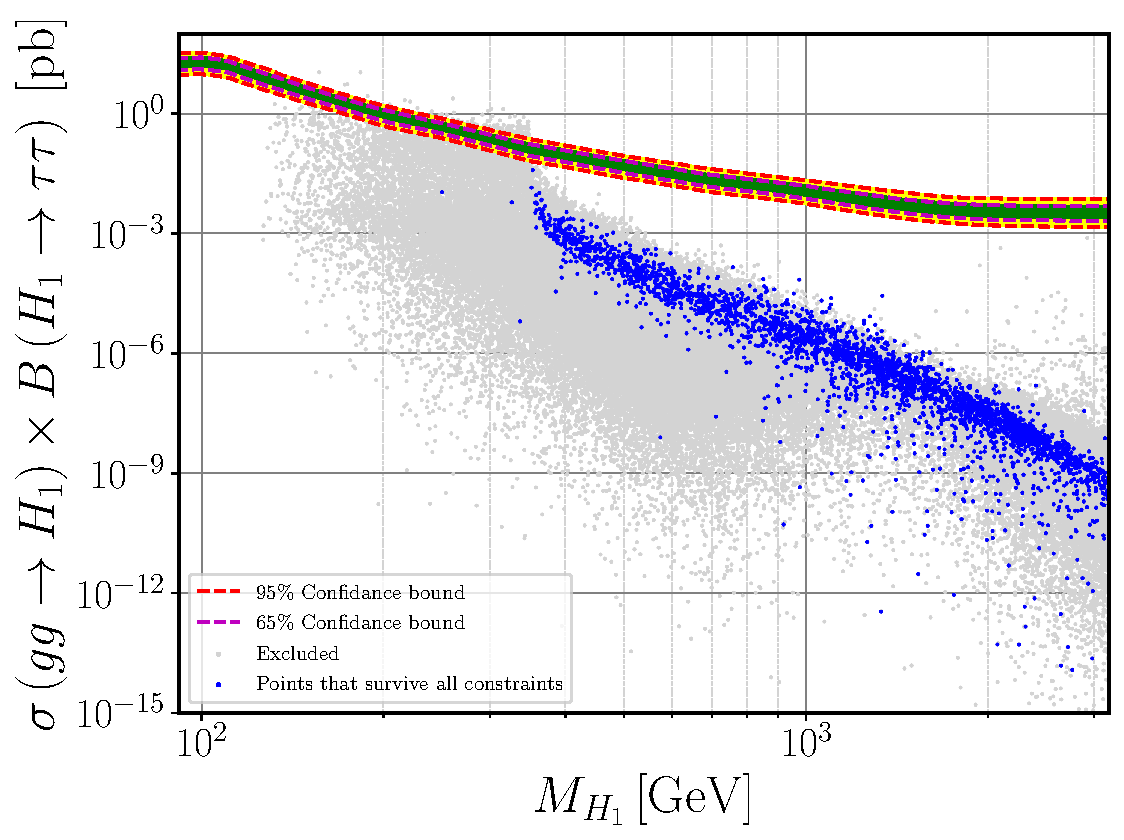
\includegraphics[width=.49\textwidth]{Images/3HDM/Xsec/Xsec_1_Grey_tight.pdf}	%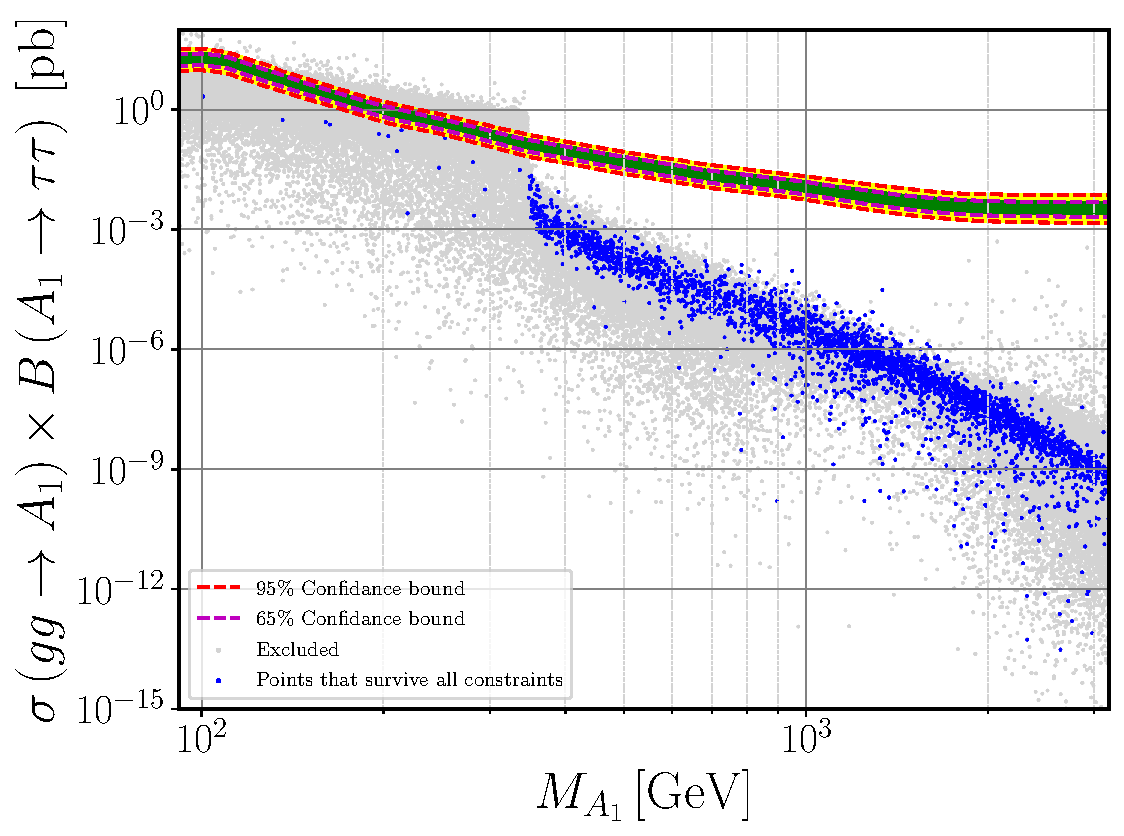
\includegraphics[width=.49\textwidth]{Images/3HDM/Xsec/Xsec_2_Colourful_tight.pdf}
	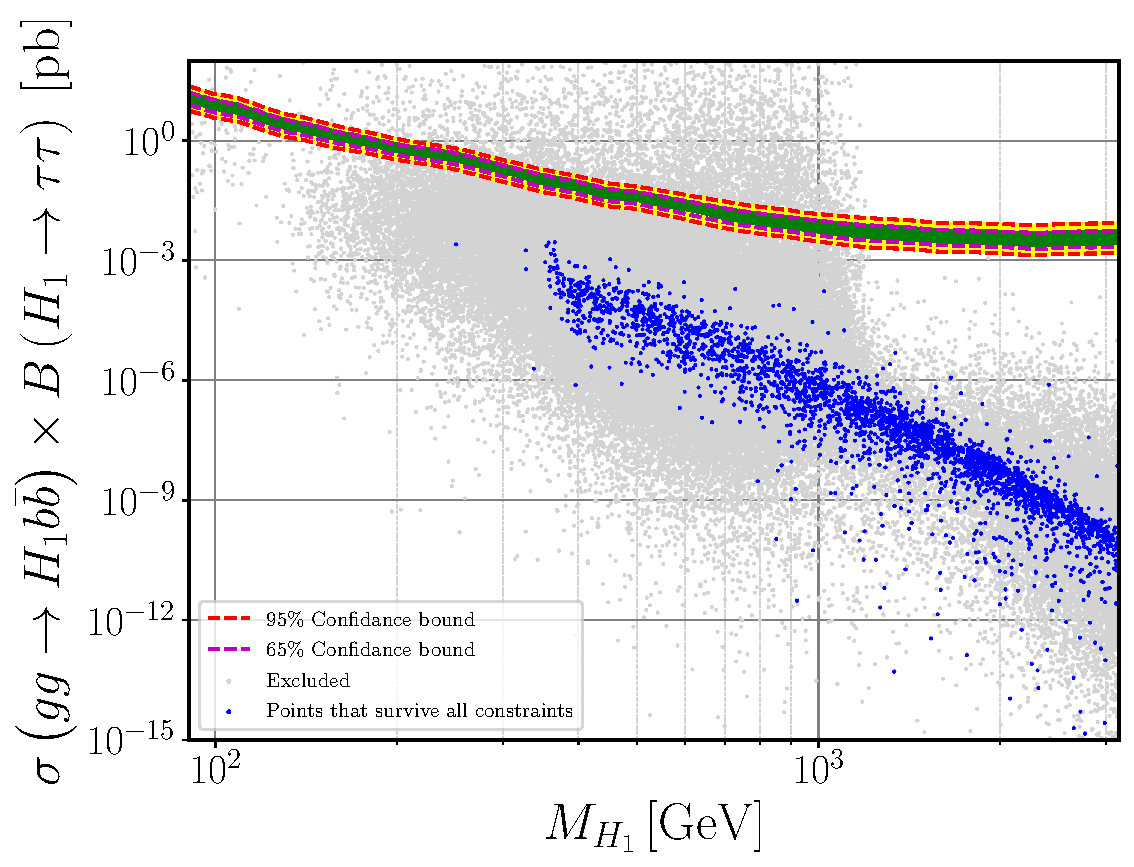
\includegraphics[width=.49\textwidth]{Images/3HDM/Xsec/Xsec_3_Grey_Thight.pdf}
	\caption{}
	\label{}
\end{figure}	
%
With these plots we can see that not only the region is clearly all bellow detection validating HiggsBounds, as we can also see there is space left to be probed at new colider experiments, both near and far from detection. 
%
This means we could be close to a new signature detection at the LHC trough gluon fusion.  

%We can see that there is still plenty of space left to be probed at new versions of the LHC and that the surviving scalars could possibly remain elusive for the considered processes, 


